% Options for packages loaded elsewhere
\PassOptionsToPackage{unicode}{hyperref}
\PassOptionsToPackage{hyphens}{url}
\PassOptionsToPackage{dvipsnames,svgnames,x11names}{xcolor}
%
\documentclass[
  letterpaper,
  DIV=11,
  numbers=noendperiod]{scrreport}

\usepackage{amsmath,amssymb}
\usepackage{lmodern}
\usepackage{iftex}
\ifPDFTeX
  \usepackage[T1]{fontenc}
  \usepackage[utf8]{inputenc}
  \usepackage{textcomp} % provide euro and other symbols
\else % if luatex or xetex
  \usepackage{unicode-math}
  \defaultfontfeatures{Scale=MatchLowercase}
  \defaultfontfeatures[\rmfamily]{Ligatures=TeX,Scale=1}
\fi
% Use upquote if available, for straight quotes in verbatim environments
\IfFileExists{upquote.sty}{\usepackage{upquote}}{}
\IfFileExists{microtype.sty}{% use microtype if available
  \usepackage[]{microtype}
  \UseMicrotypeSet[protrusion]{basicmath} % disable protrusion for tt fonts
}{}
\makeatletter
\@ifundefined{KOMAClassName}{% if non-KOMA class
  \IfFileExists{parskip.sty}{%
    \usepackage{parskip}
  }{% else
    \setlength{\parindent}{0pt}
    \setlength{\parskip}{6pt plus 2pt minus 1pt}}
}{% if KOMA class
  \KOMAoptions{parskip=half}}
\makeatother
\usepackage{xcolor}
\setlength{\emergencystretch}{3em} % prevent overfull lines
\setcounter{secnumdepth}{5}
% Make \paragraph and \subparagraph free-standing
\ifx\paragraph\undefined\else
  \let\oldparagraph\paragraph
  \renewcommand{\paragraph}[1]{\oldparagraph{#1}\mbox{}}
\fi
\ifx\subparagraph\undefined\else
  \let\oldsubparagraph\subparagraph
  \renewcommand{\subparagraph}[1]{\oldsubparagraph{#1}\mbox{}}
\fi


\providecommand{\tightlist}{%
  \setlength{\itemsep}{0pt}\setlength{\parskip}{0pt}}\usepackage{longtable,booktabs,array}
\usepackage{calc} % for calculating minipage widths
% Correct order of tables after \paragraph or \subparagraph
\usepackage{etoolbox}
\makeatletter
\patchcmd\longtable{\par}{\if@noskipsec\mbox{}\fi\par}{}{}
\makeatother
% Allow footnotes in longtable head/foot
\IfFileExists{footnotehyper.sty}{\usepackage{footnotehyper}}{\usepackage{footnote}}
\makesavenoteenv{longtable}
\usepackage{graphicx}
\makeatletter
\def\maxwidth{\ifdim\Gin@nat@width>\linewidth\linewidth\else\Gin@nat@width\fi}
\def\maxheight{\ifdim\Gin@nat@height>\textheight\textheight\else\Gin@nat@height\fi}
\makeatother
% Scale images if necessary, so that they will not overflow the page
% margins by default, and it is still possible to overwrite the defaults
% using explicit options in \includegraphics[width, height, ...]{}
\setkeys{Gin}{width=\maxwidth,height=\maxheight,keepaspectratio}
% Set default figure placement to htbp
\makeatletter
\def\fps@figure{htbp}
\makeatother
\newlength{\cslhangindent}
\setlength{\cslhangindent}{1.5em}
\newlength{\csllabelwidth}
\setlength{\csllabelwidth}{3em}
\newlength{\cslentryspacingunit} % times entry-spacing
\setlength{\cslentryspacingunit}{\parskip}
\newenvironment{CSLReferences}[2] % #1 hanging-ident, #2 entry spacing
 {% don't indent paragraphs
  \setlength{\parindent}{0pt}
  % turn on hanging indent if param 1 is 1
  \ifodd #1
  \let\oldpar\par
  \def\par{\hangindent=\cslhangindent\oldpar}
  \fi
  % set entry spacing
  \setlength{\parskip}{#2\cslentryspacingunit}
 }%
 {}
\usepackage{calc}
\newcommand{\CSLBlock}[1]{#1\hfill\break}
\newcommand{\CSLLeftMargin}[1]{\parbox[t]{\csllabelwidth}{#1}}
\newcommand{\CSLRightInline}[1]{\parbox[t]{\linewidth - \csllabelwidth}{#1}\break}
\newcommand{\CSLIndent}[1]{\hspace{\cslhangindent}#1}

\usepackage{amsmath}
\usepackage{booktabs}
\usepackage{caption}
\usepackage{longtable}
\KOMAoption{captions}{tableheading}
\makeatletter
\makeatother
\makeatletter
\@ifpackageloaded{bookmark}{}{\usepackage{bookmark}}
\makeatother
\makeatletter
\@ifpackageloaded{caption}{}{\usepackage{caption}}
\AtBeginDocument{%
\ifdefined\contentsname
  \renewcommand*\contentsname{Table of contents}
\else
  \newcommand\contentsname{Table of contents}
\fi
\ifdefined\listfigurename
  \renewcommand*\listfigurename{List of Figures}
\else
  \newcommand\listfigurename{List of Figures}
\fi
\ifdefined\listtablename
  \renewcommand*\listtablename{List of Tables}
\else
  \newcommand\listtablename{List of Tables}
\fi
\ifdefined\figurename
  \renewcommand*\figurename{Figure}
\else
  \newcommand\figurename{Figure}
\fi
\ifdefined\tablename
  \renewcommand*\tablename{Table}
\else
  \newcommand\tablename{Table}
\fi
}
\@ifpackageloaded{float}{}{\usepackage{float}}
\floatstyle{ruled}
\@ifundefined{c@chapter}{\newfloat{codelisting}{h}{lop}}{\newfloat{codelisting}{h}{lop}[chapter]}
\floatname{codelisting}{Listing}
\newcommand*\listoflistings{\listof{codelisting}{List of Listings}}
\makeatother
\makeatletter
\@ifpackageloaded{caption}{}{\usepackage{caption}}
\@ifpackageloaded{subcaption}{}{\usepackage{subcaption}}
\makeatother
\makeatletter
\@ifpackageloaded{tcolorbox}{}{\usepackage[many]{tcolorbox}}
\makeatother
\makeatletter
\@ifundefined{shadecolor}{\definecolor{shadecolor}{rgb}{.97, .97, .97}}
\makeatother
\makeatletter
\makeatother
\ifLuaTeX
  \usepackage{selnolig}  % disable illegal ligatures
\fi
\IfFileExists{bookmark.sty}{\usepackage{bookmark}}{\usepackage{hyperref}}
\IfFileExists{xurl.sty}{\usepackage{xurl}}{} % add URL line breaks if available
\urlstyle{same} % disable monospaced font for URLs
\hypersetup{
  pdftitle={Regression without regrets},
  pdfauthor={M. Baillie, G. Heinze \& M. Huebner},
  colorlinks=true,
  linkcolor={blue},
  filecolor={Maroon},
  citecolor={Blue},
  urlcolor={Blue},
  pdfcreator={LaTeX via pandoc}}

\title{Regression without regrets}
\author{M. Baillie, G. Heinze \& M. Huebner}
\date{11/17/22}

\begin{document}
\maketitle
\ifdefined\Shaded\renewenvironment{Shaded}{\begin{tcolorbox}[frame hidden, interior hidden, sharp corners, borderline west={3pt}{0pt}{shadecolor}, boxrule=0pt, enhanced, breakable]}{\end{tcolorbox}}\fi

\renewcommand*\contentsname{Table of contents}
{
\hypersetup{linkcolor=}
\setcounter{tocdepth}{2}
\tableofcontents
}
\bookmarksetup{startatroot}

\hypertarget{preface}{%
\chapter*{Preface}\label{preface}}
\addcontentsline{toc}{chapter}{Preface}

\markboth{Preface}{Preface}

The draft report is work in progress.

The focus of this site is to provide guidance on conducting initial data
analysis in a reproducible manner in the context of intended regression
analyses.

\bookmarksetup{startatroot}

\hypertarget{Bacteremia}{%
\chapter{Bacteremia study}\label{Bacteremia}}

\hypertarget{overview-of-the-bacteremia-study}{%
\section{Overview of the bacteremia
study}\label{overview-of-the-bacteremia-study}}

We will exemplify our proposed systematic approach to data screening by
means of a diagnostic study with the primary aim of using age, sex and
49 laboratory variables to fit a diagnostic prediction model for the
bacteremia status (= presence of bacteria in the blood stream) of a
blood sample. A secondary aim of the study is to describe the functional
form of each predictor in the model. Between January 2006 and December
2010, patients with the clinical suspicion to suffer from bacteremia
were included if blood culture analysis was requested by the responsible
physician and blood was sampled for assessment of hematology and
biochemistry. An analysis of this study can be found in Ratzinger et al:
``A Risk Prediction Model for Screening Bacteremic Patients: A Cross
Sectional Study''
\href{https://doi.org/10.1371/journal.pone.0106765}{Ratzinger et al.
(2014)}.

The data consists of 14,691 observations from different patients and 51
potential predictors. To protect data privacy our version of this data
was slightly modified compared to the original version, and this
modified version was cleared by the Medical University of Vienna for
public use (DC 2019-0054). Compared to the official results given in
(Ratzinger et al. 2014), our results may differ to a negligible degree.

\hypertarget{source-dataset}{%
\subsection{Source dataset}\label{source-dataset}}

We refer to the \textbf{source} data as the data set available in this
repository. First we read and display the data dictionary to provide an
overview of the collected measurements.

\captionsetup[table]{labelformat=empty,skip=1pt}
\begin{longtable}{rllllll}
\toprule
variable\_nr & variable & label & scale\_of\_measurement & units & remark & from\_paper \\ 
\midrule
1 & ID & Patient Identification & nominal & 1-14691 & NA & NA \\ 
2 & SEX & Patient sex & nominal & 1=male, 2=female & NA & Female: Male \\ 
3 & AGE & Patient Age & continuous & years & Alter=German age & Albumin (G/L) 14,187 33.7 (28?39.3) 32 (26.925?36.7) ,0.0001 0.568 \\ 
4 & MCV & Mean corpuscular volume & continuous & pg & NA & MCV (pg) 15,941 88.1 (84.6?91.9) 88.6 (84.8?92.5) 0.0044 0.524 \\ 
5 & HGB & Haemoglobin & continuous & G/L & NA & Haemoglobin(G/L) 15,942 11.4 (9.9?13.2) 11.1 (9.5?12.6) ,0.0001 0.554 \\ 
6 & HCT & Haematocrit & continuous & \% & NA & Haematocrit (\%) 15,941 34.4 (29.8?39.2) 33.1 (28.5?37.5) ,0.0001 0.561 \\ 
7 & PLT & Blood platelets & continuous & G/L & NA & PLT (G/L) 15,940 206 (142?279.25) 180.5 (115?248) ,0.0001 0.575 \\ 
8 & MCH & Mean corpuscular hemoglobin & continuous & fl & NA & MCH (fl) 15,941 29.7 (28.3?30.9) 29.8 (28.5?31.2) 0.0019 0.526 \\ 
9 & MCHC & Mean corpuscular hemoglobin concentration & continuous & g/dl & NA & MCHC (g/dl) 15,941 33.5 (32.6?34.4) 33.6 (32.7?34.5) n.s. \\ 
10 & RDW & Red blood cell distribution width & continuous & \% & NA & RDW (\%) 15,924 14.4 (13.3?15.925) 14.9 (13.7?16.6) ,0.0001 0.572 \\ 
11 & MPV & Mean platelet volume & continuous & fl & NA & MPV (fl) 15,214 10.3 (9.7?11) 10.4 (9.7?11.1) n.s. \\ 
12 & LYM & Lymphocytes & continuous & G/L & NA & Lymphocytes (G/L) 15,695 1.1 (0.7?1.6) 0.7 (0.4?1.1) ,0.0001 0.683 \\ 
13 & MONO & Monocytes & continuous & G/L & NA & Monocytes (G/L) 15,710 0.8 (0.5?1.1) 0.6 (0.3?1) ,0.0001 0.598 \\ 
14 & EOS & Eosinophils & continuous & G/L & NA & Eosinophils (G/L) 15,373 0.6 (0.1?1.8) 0.2 (0?0.8) ,0.0001 0.641 \\ 
15 & BASO & Basophiles & continuous & G/L & NA & Basophiles \% 15,375 0.2 (0.1?0.3) 0.1 (0.1?0.2) ,0.0001 0.606 \\ 
16 & NT & Normotest & continuous & \% & Measures thromboplastin time & Normotest (\%) 13,339 84 (67?101) 78 (60?94) ,0.0001 0.571 \\ 
17 & APTT & Activated partial thromboplastin time & continuous & sec & NA & aPTT (sec) 13,251 37.8 (34.2?42.8) 37.8 (34.2?43) n.s. \\ 
18 & FIB & Fibrinogen & continuous & mg/dl & NA & Fibrinogen (mg/dl) 13,211 526 (393?667) 546 (424?701) 0.0001 0.538 \\ 
19 & SODIUM & Sodium & continuous & mmol/L & Natrium=German sodium & Sodium (mmol/L) 14,542 138 (135?140) 136 (133?139) ,0.0001 0.602 \\ 
20 & POTASS & Potassium & continuous & mmol/L & NA & Potassium (mmol/L) 13,774 3.95 (3.67?4.3) 3.97 (3.595?4.365) n.s. \\ 
21 & CA & Calcium & continuous & mmol/L & NA & Calcium (mmol/L) 14,592 2.23 (2.09?2.35) 2.21 (2.08?2.33) 0.0001 0.533 \\ 
22 & PHOS & Phosphate & continuous & mmol/L & NA & Phosphate(mmol/L) 14,664 1 (0.81?1.2) 0.95 (0.76?1.19) ,0.0001 0.537 \\ 
23 & MG & Magnesium & continuous & mmol/L & NA & MG (mmol/L) 13,989 0.81 (0.73?0.89) 0.77 (0.68?0.86) ,0.0001 0.582 \\ 
24 & CREA & Creatinine & continuous & mg/dl & NA & Creatinine (mg/dl) 15,813 0.99 (0.81?1.31) 1.2 (0.89?1.87) ,0.0001 0.611 \\ 
25 & BUN & Blood urea nitrogen & continuous & mg/dl & NA & BUN (mg/dl) 15,800 16.2 (11.4?25.8) 22.5 (14.7?37.78) ,0.0001 0.633 \\ 
26 & HS & Uric acid & continuous & mg/dl & Harns?ure=German Uric acid & Uric acid (mg/dl) 12,709 5 (3.7?6.5) 5.5 (3.9?7.6) ,0.0001 0.562 \\ 
27 & GBIL & Bilirubin & continuous & mg/dl & NA & Bilirubin (mg/dl) 14,431 0.75 (0.52?1.19) 1.02 (0.66?1.73) ,0.0001 0.621 \\ 
28 & TP & Total protein & continuous & G/L & NA & TP (G/L) 14,301 65.8 (56.8?73.4) 64.7 (56.4?71.5) 0.0019 0.528 \\ 
29 & ALB & Albumin & continuous & G/L & NA & ALAT (U/L) 14,919 26 (16?47) 30 (18?60) ,0.0001 0.55 \\ 
30 & AMY & Amylase & continuous & U/L & NA & Amylase (U/L) 11,783 50 (34?77) 44 (28?70) ,0.0001 0.565 \\ 
31 & PAMY & Pancreas amylase & continuous & U/L & NA & PAMY (U/L) \\ 
32 & LIP & Lipases & continuous & U/L & NA & Lipases (U/L) 11,988 23 (13?40) 22 (12?38) n.s. \\ 
33 & CHE & Cholinesterase & continuous & kU/L & NA & CHE (kU/L) 13,353 4.66 (3.2?6.29) 3.94 (2.66?5.48) ,0.0001 0.591 \\ 
34 & AP & Alkaline phosphatase & continuous & U/L & NA & ALP (U/L) 14,479 83 (62?120) 100 (72?164) ,0.0001 0.601 \\ 
35 & ASAT & Aspartate transaminase & continuous & U/L & NA & ASAT (U/L) 14,745 31 (22?56) 37 (24?70.25) ,0.0001 0.558 \\ 
36 & ALAT & Alanin transaminase & continuous & U/L & NA & Age 15,985 58 (42?69) 65 (53?74) ,0.0001 0.611 \\ 
37 & GGT & Gamma-glutamyl transpeptidase & continuous & G/L & NA & GGT (G/L) 14,629 48 (25?112) 73 (35?180) ,0.0001 0.599 \\ 
38 & LDH & Lactate dehydrogenase & continuous & U/L & NA & LDH (U/L) 14,150 239 (186?334) 249 (199?331.5) 0.0037 0.527 \\ 
39 & CK & Creatinine kinases & continuous & U/L & NA & CK (U/L) 13,763 82 (42?190) 67 (34?142) ,0.0001 0.557 \\ 
40 & GLU & Glucoses & continuous & mg/dl & NA & Glucoses (mg/dl) 11,350 113 (96?137) 121 (99?154) ,0.0001 0.559 \\ 
41 & TRIG & Triclyceride & continuous & mg/dl & NA & Triglyceride (mg/dl) 10,549 115 (83?164) 118 (85?170) n.s. \\ 
42 & CHOL & Cholesterol & continuous & mg/dl & NA & Cholesterol (mg/dl) 10,565 146 (114?183) 132 (105?171) ,0.0001 0.564 \\ 
43 & CRP & C-reactive protein & continuous & mg/dl & NA & CRP (mg/dl) 15,820 8.39 (2.77?16.15) 11.68 (5.22?21.19) ,0.0001 0.596 \\ 
44 & BASOR & Basophile ratio & continuous & \% & NA & Basophiles (G/L) 15,827 0 (0?0) 0 (0?0) ,0.0001 0.47 \\ 
45 & EOSR & Eosinophil ratio & continuous & \% & NA & Eosinophil \% 15,831 0.1 (0?0.2) 0 (0?0.1) ,0.0001 0.626 \\ 
46 & LYMR & Lymphocyte ratio & continuous & \% (mg/dl) & NA & Lymphocytes \% (mg/dl) 15,250 11.6 (7.1?18.6) 7 (4.15?12.2) ,0.0001 0.674 \\ 
47 & MONOR & Monocyte ratio & continuous & \% & NA & Monocytes \% 15,268 8.1 (5.8?10.7) 6.1 (3.5?8.8) ,0.0001 0.645 \\ 
48 & NEU & Neutrophiles & continuous & G/L & NA & Neutrophiles (G/L) 15,181 7.3 (4.6?10.7) 8.4 (5.23?12.7) ,0.0001 0.559 \\ 
49 & NEUR & Neutrophile ratio & continuous & \% & NA & Neutrophiles \% 15,181 77.7 (68.7?84.6) 85.8 (78.3?90.5) ,0.0001 0.696 \\ 
50 & PDW & Platelet distribution width & continuous & \% & NA & PDW (\%) 14,776 12 (10.8?13.4) 12.1 (10.8?13.7) n.s. \\ 
51 & RBC & Red blood count & continuous & T/L & NA & RBC (T/L) 15,478 3.9 (3.4?4.5) 3.7 (3.2?4.2) ,0.0001 0.567 \\ 
52 & WBC & White blood count & continuous & G/L & NA & WBC (G/L) 15,477 9.58 (6.64?13.46) 10.205 (6.61?14.86) n.s. \\ 
53 & BloodCulture & Blood culture result for bacteremia & nominal & no, yes & NA & NA \\ 
\bottomrule
\end{longtable}

Display a short summary of the source data set contents. The source data
set is in the \textbf{data-raw} folder of the project directory.

\begin{longtable}[]{@{}lll@{}}
\toprule()
Name & Storage & NAs \\
\midrule()
\endhead
ID & double & 0 \\
SEX & double & 0 \\
AGE & double & 0 \\
MCV & double & 42 \\
HGB & double & 41 \\
HCT & double & 42 \\
PLT & double & 42 \\
MCH & double & 42 \\
MCHC & double & 42 \\
RDW & double & 56 \\
MPV & double & 702 \\
LYM & double & 262 \\
MONO & double & 246 \\
EOS & double & 135 \\
BASO & double & 146 \\
NT & double & 2467 \\
APTT & double & 2549 \\
FIB & double & 2567 \\
SODIUM & double & 1282 \\
POTASS & double & 2008 \\
CA & double & 1276 \\
PHOS & double & 1242 \\
MG & double & 1869 \\
CREA & double & 159 \\
BUN & double & 172 \\
HS & double & 3061 \\
GBIL & double & 1441 \\
TP & double & 1583 \\
ALB & double & 1676 \\
AMY & double & 3913 \\
PAMY & double & 7114 \\
LIP & double & 3699 \\
CHE & double & 2447 \\
AP & double & 1400 \\
ASAT & double & 1154 \\
ALAT & double & 987 \\
GGT & double & 1262 \\
LDH & double & 1714 \\
CK & double & 2080 \\
GLU & double & 4192 \\
TRIG & double & 5061 \\
CHOL & double & 5045 \\
CRP & double & 155 \\
BASOR & double & 732 \\
EOSR & double & 732 \\
LYMR & double & 732 \\
MONOR & double & 732 \\
NEU & double & 728 \\
NEUR & double & 732 \\
PDW & double & 1102 \\
RBC & double & 461 \\
WBC & double & 462 \\
BloodCulture & character & 0 \\
\bottomrule()
\end{longtable}

An alternative approach to displaying contents. Display the source data
dynamically.

\hypertarget{updated-analysis-dataset}{%
\subsection{Updated analysis dataset}\label{updated-analysis-dataset}}

Additional meta-data is added to the original \emph{source} data set. We
write this new modified (annotated) data set back to the \textbf{data}
folder after adding additional meta-data for all variables. The
meta-data is taken from the data dictionary. The aim is to produce an
analysis ready data set for the research objective.

At the stage we could select the variables of interest to take in to the
IDA phase by dropping variables we do not check in IDA.

As a cross check we display the contents again to ensure the additional
data is added, and then write the changes to the data folder in the file
\textbf{``data/a\_bact.rda''}.

\bookmarksetup{startatroot}

\hypertarget{IDA_plan}{%
\chapter{IDA plan}\label{IDA_plan}}

This document exemplifies the prespecified plan for initial data
analysis (IDA plan) for the bacteremia study.

\hypertarget{prerequisites-for-the-ida-plan}{%
\section{Prerequisites for the IDA
plan}\label{prerequisites-for-the-ida-plan}}

\hypertarget{analysis-strategy}{%
\subsection{Analysis strategy}\label{analysis-strategy}}

We assume that the aims of the study are to fit a diagnostic prediction
model and to describe the functional form of each predictor. These aims
are addressed by fitting a logistic regression model with bacteremia
status as the dependent variable.

Based on domain expertise, the predictors are grouped by their assumed
importance to predict bacteremia. Variables with known strong
associations with bacteremia are age (AGE), leukocytes (WBC), blood urea
neutrogen (BUN), creatinine (CREA), thrombocytes (PLT), and neutrophiles
(NEU) and these predictors will be included in the model as key
predictors. Predictors of medium importance are potassium (POTASS), and
some acute-phase related parameters such as fibrinogen (FIB), C-reactive
protein (CRP), aspartate transaminase (ASAT), alanine transaminase
(ALAT), and gamma-glutamyl transpeptidase (GGT). All other predictors
are of minor importance.

Continuous predictors should be modelled by allowing for flexible
functional forms, where for all key predictors four degrees of freedom
will be spent, and for predictors of medium and minor importance, three
or two degrees of freedom should be foreseen at maximum, respectively.
The decision on whether to use only key predictors, or to consider
predictors also from the predictor sets of medium or minor importance
depends on results of data screening, but will be made before uncovering
the association of predictors with the outcome variable.

An adequate strategy to cope with missing values will also be chosen
after screening the data. Candidate strategies are omission of
predictors with abundant missing values, complete case analysis, single
value imputation or multiple imputation with chained equations.

\hypertarget{data-dictionary}{%
\subsection{Data dictionary}\label{data-dictionary}}

The data dictionary of the bacteremia data set consists of columns for
variable names, variable labels, scale of measurement (continuous or
categorical), units, plausibility limits, and remarks:

\captionsetup[table]{labelformat=empty,skip=1pt}
\begin{longtable}{lrllllll}
\toprule
notes & variable\_nr & variable & label & scale\_of\_measurement & units & remark & from\_paper \\ 
\midrule
Source & 1 & ID & Patient Identification & nominal & 1-14691 & NA & NA \\ 
Source & 2 & SEX & Patient sex & nominal & 1=male, 2=female & NA & Female: Male \\ 
Source & 3 & AGE & Patient Age & continuous & years & Alter=German age & Albumin (G/L) 14,187 33.7 (28?39.3) 32 (26.925?36.7) ,0.0001 0.568 \\ 
Source & 4 & MCV & Mean corpuscular volume & continuous & pg & NA & MCV (pg) 15,941 88.1 (84.6?91.9) 88.6 (84.8?92.5) 0.0044 0.524 \\ 
Source & 5 & HGB & Haemoglobin & continuous & G/L & NA & Haemoglobin(G/L) 15,942 11.4 (9.9?13.2) 11.1 (9.5?12.6) ,0.0001 0.554 \\ 
Source & 6 & HCT & Haematocrit & continuous & \% & NA & Haematocrit (\%) 15,941 34.4 (29.8?39.2) 33.1 (28.5?37.5) ,0.0001 0.561 \\ 
Source & 7 & PLT & Blood platelets & continuous & G/L & NA & PLT (G/L) 15,940 206 (142?279.25) 180.5 (115?248) ,0.0001 0.575 \\ 
Source & 8 & MCH & Mean corpuscular hemoglobin & continuous & fl & NA & MCH (fl) 15,941 29.7 (28.3?30.9) 29.8 (28.5?31.2) 0.0019 0.526 \\ 
Source & 9 & MCHC & Mean corpuscular hemoglobin concentration & continuous & g/dl & NA & MCHC (g/dl) 15,941 33.5 (32.6?34.4) 33.6 (32.7?34.5) n.s. \\ 
Source & 10 & RDW & Red blood cell distribution width & continuous & \% & NA & RDW (\%) 15,924 14.4 (13.3?15.925) 14.9 (13.7?16.6) ,0.0001 0.572 \\ 
Source & 11 & MPV & Mean platelet volume & continuous & fl & NA & MPV (fl) 15,214 10.3 (9.7?11) 10.4 (9.7?11.1) n.s. \\ 
Source & 12 & LYM & Lymphocytes & continuous & G/L & NA & Lymphocytes (G/L) 15,695 1.1 (0.7?1.6) 0.7 (0.4?1.1) ,0.0001 0.683 \\ 
Source & 13 & MONO & Monocytes & continuous & G/L & NA & Monocytes (G/L) 15,710 0.8 (0.5?1.1) 0.6 (0.3?1) ,0.0001 0.598 \\ 
Source & 14 & EOS & Eosinophils & continuous & G/L & NA & Eosinophils (G/L) 15,373 0.6 (0.1?1.8) 0.2 (0?0.8) ,0.0001 0.641 \\ 
Source & 15 & BASO & Basophiles & continuous & G/L & NA & Basophiles \% 15,375 0.2 (0.1?0.3) 0.1 (0.1?0.2) ,0.0001 0.606 \\ 
Source & 16 & NT & Normotest & continuous & \% & Measures thromboplastin time & Normotest (\%) 13,339 84 (67?101) 78 (60?94) ,0.0001 0.571 \\ 
Source & 17 & APTT & Activated partial thromboplastin time & continuous & sec & NA & aPTT (sec) 13,251 37.8 (34.2?42.8) 37.8 (34.2?43) n.s. \\ 
Source & 18 & FIB & Fibrinogen & continuous & mg/dl & NA & Fibrinogen (mg/dl) 13,211 526 (393?667) 546 (424?701) 0.0001 0.538 \\ 
Source & 19 & SODIUM & Sodium & continuous & mmol/L & Natrium=German sodium & Sodium (mmol/L) 14,542 138 (135?140) 136 (133?139) ,0.0001 0.602 \\ 
Source & 20 & POTASS & Potassium & continuous & mmol/L & NA & Potassium (mmol/L) 13,774 3.95 (3.67?4.3) 3.97 (3.595?4.365) n.s. \\ 
Source & 21 & CA & Calcium & continuous & mmol/L & NA & Calcium (mmol/L) 14,592 2.23 (2.09?2.35) 2.21 (2.08?2.33) 0.0001 0.533 \\ 
Source & 22 & PHOS & Phosphate & continuous & mmol/L & NA & Phosphate(mmol/L) 14,664 1 (0.81?1.2) 0.95 (0.76?1.19) ,0.0001 0.537 \\ 
Source & 23 & MG & Magnesium & continuous & mmol/L & NA & MG (mmol/L) 13,989 0.81 (0.73?0.89) 0.77 (0.68?0.86) ,0.0001 0.582 \\ 
Source & 24 & CREA & Creatinine & continuous & mg/dl & NA & Creatinine (mg/dl) 15,813 0.99 (0.81?1.31) 1.2 (0.89?1.87) ,0.0001 0.611 \\ 
Source & 25 & BUN & Blood urea nitrogen & continuous & mg/dl & NA & BUN (mg/dl) 15,800 16.2 (11.4?25.8) 22.5 (14.7?37.78) ,0.0001 0.633 \\ 
Source & 26 & HS & Uric acid & continuous & mg/dl & Harns?ure=German Uric acid & Uric acid (mg/dl) 12,709 5 (3.7?6.5) 5.5 (3.9?7.6) ,0.0001 0.562 \\ 
Source & 27 & GBIL & Bilirubin & continuous & mg/dl & NA & Bilirubin (mg/dl) 14,431 0.75 (0.52?1.19) 1.02 (0.66?1.73) ,0.0001 0.621 \\ 
Source & 28 & TP & Total protein & continuous & G/L & NA & TP (G/L) 14,301 65.8 (56.8?73.4) 64.7 (56.4?71.5) 0.0019 0.528 \\ 
Source & 29 & ALB & Albumin & continuous & G/L & NA & ALAT (U/L) 14,919 26 (16?47) 30 (18?60) ,0.0001 0.55 \\ 
Source & 30 & AMY & Amylase & continuous & U/L & NA & Amylase (U/L) 11,783 50 (34?77) 44 (28?70) ,0.0001 0.565 \\ 
Source & 31 & PAMY & Pancreas amylase & continuous & U/L & NA & PAMY (U/L) \\ 
Source & 32 & LIP & Lipases & continuous & U/L & NA & Lipases (U/L) 11,988 23 (13?40) 22 (12?38) n.s. \\ 
Source & 33 & CHE & Cholinesterase & continuous & kU/L & NA & CHE (kU/L) 13,353 4.66 (3.2?6.29) 3.94 (2.66?5.48) ,0.0001 0.591 \\ 
Source & 34 & AP & Alkaline phosphatase & continuous & U/L & NA & ALP (U/L) 14,479 83 (62?120) 100 (72?164) ,0.0001 0.601 \\ 
Source & 35 & ASAT & Aspartate transaminase & continuous & U/L & NA & ASAT (U/L) 14,745 31 (22?56) 37 (24?70.25) ,0.0001 0.558 \\ 
Source & 36 & ALAT & Alanin transaminase & continuous & U/L & NA & Age 15,985 58 (42?69) 65 (53?74) ,0.0001 0.611 \\ 
Source & 37 & GGT & Gamma-glutamyl transpeptidase & continuous & G/L & NA & GGT (G/L) 14,629 48 (25?112) 73 (35?180) ,0.0001 0.599 \\ 
Source & 38 & LDH & Lactate dehydrogenase & continuous & U/L & NA & LDH (U/L) 14,150 239 (186?334) 249 (199?331.5) 0.0037 0.527 \\ 
Source & 39 & CK & Creatinine kinases & continuous & U/L & NA & CK (U/L) 13,763 82 (42?190) 67 (34?142) ,0.0001 0.557 \\ 
Source & 40 & GLU & Glucoses & continuous & mg/dl & NA & Glucoses (mg/dl) 11,350 113 (96?137) 121 (99?154) ,0.0001 0.559 \\ 
Source & 41 & TRIG & Triclyceride & continuous & mg/dl & NA & Triglyceride (mg/dl) 10,549 115 (83?164) 118 (85?170) n.s. \\ 
Source & 42 & CHOL & Cholesterol & continuous & mg/dl & NA & Cholesterol (mg/dl) 10,565 146 (114?183) 132 (105?171) ,0.0001 0.564 \\ 
Source & 43 & CRP & C-reactive protein & continuous & mg/dl & NA & CRP (mg/dl) 15,820 8.39 (2.77?16.15) 11.68 (5.22?21.19) ,0.0001 0.596 \\ 
Source & 44 & BASOR & Basophile ratio & continuous & \% & NA & Basophiles (G/L) 15,827 0 (0?0) 0 (0?0) ,0.0001 0.47 \\ 
Source & 45 & EOSR & Eosinophil ratio & continuous & \% & NA & Eosinophil \% 15,831 0.1 (0?0.2) 0 (0?0.1) ,0.0001 0.626 \\ 
Source & 46 & LYMR & Lymphocyte ratio & continuous & \% (mg/dl) & NA & Lymphocytes \% (mg/dl) 15,250 11.6 (7.1?18.6) 7 (4.15?12.2) ,0.0001 0.674 \\ 
Source & 47 & MONOR & Monocyte ratio & continuous & \% & NA & Monocytes \% 15,268 8.1 (5.8?10.7) 6.1 (3.5?8.8) ,0.0001 0.645 \\ 
Source & 48 & NEU & Neutrophiles & continuous & G/L & NA & Neutrophiles (G/L) 15,181 7.3 (4.6?10.7) 8.4 (5.23?12.7) ,0.0001 0.559 \\ 
Source & 49 & NEUR & Neutrophile ratio & continuous & \% & NA & Neutrophiles \% 15,181 77.7 (68.7?84.6) 85.8 (78.3?90.5) ,0.0001 0.696 \\ 
Source & 50 & PDW & Platelet distribution width & continuous & \% & NA & PDW (\%) 14,776 12 (10.8?13.4) 12.1 (10.8?13.7) n.s. \\ 
Source & 51 & RBC & Red blood count & continuous & T/L & NA & RBC (T/L) 15,478 3.9 (3.4?4.5) 3.7 (3.2?4.2) ,0.0001 0.567 \\ 
Source & 52 & WBC & White blood count & continuous & G/L & NA & WBC (G/L) 15,477 9.58 (6.64?13.46) 10.205 (6.61?14.86) n.s. \\ 
Source & 53 & BloodCulture & Blood culture result for bacteremia & nominal & no, yes & NA & NA \\ 
Dervived & 54 & BC & bacteremia & factor & 0, 1 & NA & Convert BloodCulture into a numeric factor \\ 
\bottomrule
\end{longtable}

\hypertarget{domain-expertise}{%
\subsection{Domain expertise}\label{domain-expertise}}

The demographic variables age and sex are are chosen as the structural
variables in this analysis for illustration purposes, since they are
commonly considered important for describing a cohort in health studies.
Key predictors and predictors of medium importance are as defined above.
Laboratory analyses always bear the risk of machine failures, and hence
missing values are a frequent challenge. This may differ between
laboratory variables, but no a priori estimate about the expected
proportion of missing values can be assumed. As most predictors measure
concentrations of chemical compounds or cell counts, skewed
distributions are expected. Some predictors describe related types of
cells or chemical compounds, and hence some correlation between them is
to be expected. For example, leukocytes consist of five different types
of blood cells (BASO, EOS, NEU, LYM and MONO), and the sum of the
concentration of these types approximately (but not exactly) gives the
leukocyte count, which is recorded in the variable WBC. Moreover, these
variables are given as absolute counts and as percentages of the sum of
the five variables, which creates some correlation. Some laboratory
variables differ by sex and age, but the special selection of patients
for this study (suspicion of bacteremia) may distort or alter the
expected correlations with sex and age.

For the purpose of stratifying IDA results by age, age will be
categorized into the following three groups: (16, 50{]}, (50, 65{]},
(65, 101{]}.

The predictor grouping is defined here:

\hypertarget{ida-plan}{%
\section{IDA plan}\label{ida-plan}}

\hypertarget{m1-prevalence-of-missing-values}{%
\subsection{M1: Prevalence of missing
values}\label{m1-prevalence-of-missing-values}}

Numbers and proportions of missing values will be reported for each
predictor separately (M1). Type of missingness has not been recorded.

\hypertarget{m2-complete-cases}{%
\subsection{M2: Complete cases}\label{m2-complete-cases}}

The number of available complete cases (outcome and predictors) will be
reported when considering:

\begin{enumerate}
\def\labelenumi{\arabic{enumi}.}
\tightlist
\item
  the outcome variable (BC)
\item
  outcome and structural variables (BC, AGE, SEX)
\item
  outcome and key predictors only (BC, AGE, WBC, BUN, CREA, PLT, NEU)
\item
  outcome, key predictors and predictors of medium importance (BC, AGE,
  WBC, BUN, CREA, PLT, NEU, POTASS, FIB, CRP, ASAT, ALAT, GGT)
\item
  outcome and all predictors.
\end{enumerate}

\hypertarget{m3-patterns-of-missing-values}{%
\subsection{M3: Patterns of missing
values}\label{m3-patterns-of-missing-values}}

Patterns of missing values will be investigated by:

\begin{enumerate}
\def\labelenumi{\arabic{enumi}.}
\tightlist
\item
  computing a table of complete cases (for the three predictor sets
  described above) for strata defined by the structural variables age
  and sex,
\item
  constructing a dendrogram of missing values to explore which
  predictors tend to be missing together.
\end{enumerate}

\hypertarget{u1-univariate-descriptions-categorical-variables}{%
\subsection{U1: Univariate descriptions: categorical
variables}\label{u1-univariate-descriptions-categorical-variables}}

For sex and bacteremia status, the frequency and proportion of each
category will be described numerically.

\hypertarget{u2-univariate-descriptions-continuous-variables}{%
\subsection{U2: Univariate descriptions: continuous
variables}\label{u2-univariate-descriptions-continuous-variables}}

For all continuous predictors, combo plots consisting of high-resolution
histograms, boxplots and dotplots will be created. Because of the
expected skew distribution, combo plots will also be created for
log-transformed predictors.

As numerical summaries, minimum and maximum values, main quantiles (5th,
10th, 25th, 50th, 75th, 90th, 95th), and the first four moments (mean,
standard deviation, skewness, curtosis) will be reported. The number of
distinct values and the five most frequent values will be given, as well
as the concentration ratio (ratio of frequency of most frequent value
and mean frequency of each unique value).

Graphical and parametric multivariate analyses of the predictor space
such as cluster analyses or the computation of variance inflation
factors are heavily influenced by the distribution of the predictors. In
order to make this set of analyses more robust to highly influential
points or areas of the predictor support, some predictors may need
transformation (e.g.~logarithmic). We will compute the correlation of
the untransformed and log-transformed predictors with normal deviates.
Since some predictors may have values at or close to 0, we will consider
the pseudolog transformation
\(f(x;\sigma) = sinh^{-1}(x/2\sigma)/\log10\) (Johnson, 1949) which
provides a smooth transition from linear (close to 0) to logarithmic
(further away from 0). The transformation has a parameter \(\sigma\)
which we will optimize separately for each predictor in order to achieve
an optimal approximation to a normal distribution monitored via the
correlation of normal deviates with the transformed predictor. For those
predictors for which the pseudolog-transformation increases correlation
with normal deviates by at least 0.2 units of the correlation
coefficient, the pseudolog-transformed predictor will be used in
multivariate IDA instead of the respective original predictor. For those
predictors, histograms and boxplots will be provided on both the
original and the transformed scale.

\hypertarget{v1-multivariate-descriptions-associations-of-predictors-with-structural-variables}{%
\subsection{V1: Multivariate descriptions: associations of predictors
with structural
variables}\label{v1-multivariate-descriptions-associations-of-predictors-with-structural-variables}}

A scatterplot of each predictor with age, with different panels for
males and females will be constructed. Associated Spearman correlation
coefficients will be computed.

\hypertarget{v2-multivariate-descriptions-correlation-analyses}{%
\subsection{V2: Multivariate descriptions: correlation
analyses}\label{v2-multivariate-descriptions-correlation-analyses}}

A matrix of Spearman correlation coefficients between all pairs of
predictors will be computed and described numerically as well as by
means of a heatmap.

\hypertarget{ve1-multivariate-descriptions-comparing-nonparametric-and-parametric-predictor-correlation}{%
\subsection{VE1: Multivariate descriptions: comparing nonparametric and
parametric predictor
correlation}\label{ve1-multivariate-descriptions-comparing-nonparametric-and-parametric-predictor-correlation}}

A matrix of Pearson correlation coefficients will be computed. Predictor
pairs for which Spearman and Pearson correlation coefficients differ by
more than 0.1 correlation units will be depicted in scatterplots.

\hypertarget{ve2-variable-clustering}{%
\subsection{VE2: Variable clustering}\label{ve2-variable-clustering}}

A variable clustering analysis will be performed to evaluate which
predictors are closely associated. A dendrogram groups predictors by
their correlation. Scatterplots of pairs of predictors with Spearman
correlation coefficients greater than 0.8 will be created.

\hypertarget{ve3-redundancy}{%
\subsection{VE3: Redundancy}\label{ve3-redundancy}}

Variance inflation factors will be computed between the candidate
predictors. This will be done for the three possible candidate models,
and using all complete cases in the respective candidate predictor sets.
Redundancy will further be explored by computing parametric additive
models for each predictor in the three candidate models.

\bookmarksetup{startatroot}

\hypertarget{Missing}{%
\chapter{Results of IDA: Missing values}\label{Missing}}

\hypertarget{m1-prevalence-of-missing-values-1}{%
\section{M1: Prevalence of missing
values}\label{m1-prevalence-of-missing-values-1}}

Number and percentage of missingness for each predictor, sorted by
descending missingness proportion.

\captionsetup[table]{labelformat=empty,skip=1pt}
\begin{longtable}{lrr}
\toprule
\textbf{Variable} & \textbf{Missing (count)} & \textbf{Missing (\%)} \\ 
\midrule
PAMY & 7114 & $48.42$ \\ 
TRIG & 5061 & $34.45$ \\ 
CHOL & 5045 & $34.34$ \\ 
GLU & 4192 & $28.53$ \\ 
AMY & 3913 & $26.64$ \\ 
LIP & 3699 & $25.18$ \\ 
HS & 3061 & $20.84$ \\ 
FIB & 2567 & $17.47$ \\ 
APTT & 2549 & $17.35$ \\ 
NT & 2467 & $16.79$ \\ 
CHE & 2447 & $16.66$ \\ 
CK & 2080 & $14.16$ \\ 
POTASS & 2008 & $13.67$ \\ 
MG & 1869 & $12.72$ \\ 
LDH & 1714 & $11.67$ \\ 
ALB & 1676 & $11.41$ \\ 
TP & 1583 & $10.78$ \\ 
GBIL & 1441 & $9.81$ \\ 
AP & 1400 & $9.53$ \\ 
SODIUM & 1282 & $8.73$ \\ 
CA & 1276 & $8.69$ \\ 
GGT & 1262 & $8.59$ \\ 
PHOS & 1242 & $8.45$ \\ 
ASAT & 1154 & $7.86$ \\ 
PDW & 1102 & $7.50$ \\ 
ALAT & 987 & $6.72$ \\ 
BASOR & 732 & $4.98$ \\ 
EOSR & 732 & $4.98$ \\ 
LYMR & 732 & $4.98$ \\ 
MONOR & 732 & $4.98$ \\ 
NEUR & 732 & $4.98$ \\ 
NEU & 728 & $4.96$ \\ 
MPV & 702 & $4.78$ \\ 
WBC & 462 & $3.14$ \\ 
RBC & 461 & $3.14$ \\ 
LYM & 262 & $1.78$ \\ 
MONO & 246 & $1.67$ \\ 
BUN & 172 & $1.17$ \\ 
CREA & 159 & $1.08$ \\ 
CRP & 155 & $1.06$ \\ 
BASO & 146 & $0.99$ \\ 
EOS & 135 & $0.92$ \\ 
RDW & 56 & $0.38$ \\ 
MCV & 42 & $0.29$ \\ 
HCT & 42 & $0.29$ \\ 
PLT & 42 & $0.29$ \\ 
MCH & 42 & $0.29$ \\ 
MCHC & 42 & $0.29$ \\ 
HGB & 41 & $0.28$ \\ 
SEX & 0 & $0.00$ \\ 
AGE & 0 & $0.00$ \\ 
BloodCulture & 0 & $0.00$ \\ 
GENDER & 0 & $0.00$ \\ 
AGEGROUP & 0 & $0.00$ \\ 
\bottomrule
\end{longtable}

\hypertarget{m2-complete-cases-1}{%
\section{M2: Complete cases}\label{m2-complete-cases-1}}

Number of available complete cases (outcome and predictors):

\captionsetup[table]{labelformat=empty,skip=1pt}
\begin{longtable}{lrr}
\toprule
\textbf{Set} & \textbf{Complete (count)} & \textbf{Complete (\%)} \\ 
\midrule
Outcome & 14691 & $100.00$ \\ 
Outcome\_and\_structural\_variables & 14691 & $100.00$ \\ 
Outcome\_and\_key\_predictors\_only & 13793 & $93.89$ \\ 
Outcome\_key\_predictors\_and\_predictors\_of\_medium\_importance & 9389 & $63.91$ \\ 
Outcome\_and\_all\_predictors & 3979 & $27.08$ \\ 
\bottomrule
\end{longtable}

\hypertarget{me1-patterns-of-missing-values}{%
\section{ME1: Patterns of missing
values}\label{me1-patterns-of-missing-values}}

\hypertarget{complete-cases-by-strata-defined-by-structural-variables}{%
\subsection{Complete cases by strata defined by structural
variables}\label{complete-cases-by-strata-defined-by-structural-variables}}

\captionsetup[table]{labelformat=empty,skip=1pt}
\begin{longtable}{lrr}
\toprule
\textbf{Set} & \textbf{Complete (count)} & \textbf{Complete (\%)} \\ 
\midrule
\multicolumn{1}{l}{female - 2:(50,65]} \\ 
\midrule
All\_predictors & 411 & $26.03$ \\ 
Structural\_variables & 1579 & $100.00$ \\ 
Key\_predictors & 1468 & $92.97$ \\ 
Key\_and\_medium\_importance\_predictors & 1009 & $63.90$ \\ 
\midrule
\multicolumn{1}{l}{male - 3:(65,101]} \\ 
\midrule
All\_predictors & 843 & $28.46$ \\ 
Structural\_variables & 2962 & $100.00$ \\ 
Key\_predictors & 2793 & $94.29$ \\ 
Key\_and\_medium\_importance\_predictors & 1893 & $63.91$ \\ 
\midrule
\multicolumn{1}{l}{male - 1:(15,50]} \\ 
\midrule
All\_predictors & 805 & $27.73$ \\ 
Structural\_variables & 2903 & $100.00$ \\ 
Key\_predictors & 2744 & $94.52$ \\ 
Key\_and\_medium\_importance\_predictors & 1879 & $64.73$ \\ 
\midrule
\multicolumn{1}{l}{female - 1:(15,50]} \\ 
\midrule
All\_predictors & 604 & $24.53$ \\ 
Structural\_variables & 2462 & $100.00$ \\ 
Key\_predictors & 2309 & $93.79$ \\ 
Key\_and\_medium\_importance\_predictors & 1564 & $63.53$ \\ 
\midrule
\multicolumn{1}{l}{male - 2:(50,65]} \\ 
\midrule
All\_predictors & 771 & $28.87$ \\ 
Structural\_variables & 2671 & $100.00$ \\ 
Key\_predictors & 2504 & $93.75$ \\ 
Key\_and\_medium\_importance\_predictors & 1742 & $65.22$ \\ 
\midrule
\multicolumn{1}{l}{female - 3:(65,101]} \\ 
\midrule
All\_predictors & 545 & $25.78$ \\ 
Structural\_variables & 2114 & $100.00$ \\ 
Key\_predictors & 1975 & $93.42$ \\ 
Key\_and\_medium\_importance\_predictors & 1302 & $61.59$ \\ 
\bottomrule
\end{longtable}

\hypertarget{dendrogram-of-missingness-indicators}{%
\subsection{Dendrogram of missingness
indicators}\label{dendrogram-of-missingness-indicators}}

The dendrogram depicts the results of a cluster analysis using the
complete linkage method based on the percentage of discordant missing
indicators. (This percentage was computed via the squared Euclidian
distance of missingness indicators between predictors.) The vertical
axis shows the distance between two clusters, which is given by the
maximum distance between any element of the first and the second
clusters. For example, if two clusters are merged at a height of 25 it
means that in 25\% of the observations the missingness indicators of the
most discordant predictors contained in the two clusters are discordant.

The numbers in brackets are the percentages of missing observations for
each predictor.

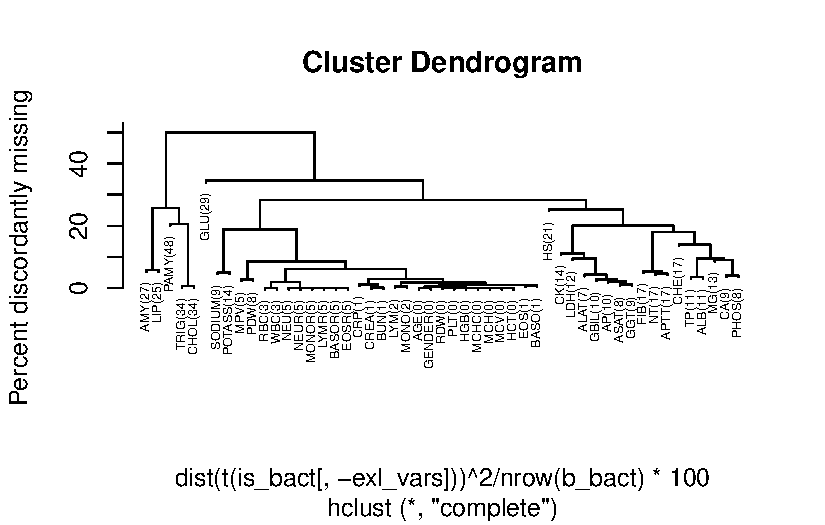
\includegraphics{./Bact_missing_files/figure-pdf/unnamed-chunk-5-1.pdf}

\bookmarksetup{startatroot}

\hypertarget{univariate-distribution-checks}{%
\chapter{Univariate distribution
checks}\label{univariate-distribution-checks}}

This section reports a series of univariate summary checks of the
bacteremia dataset.

\hypertarget{u1-categorical-variables}{%
\section{U1: Categorical variables}\label{u1-categorical-variables}}

SEX and BC (bactermia status) are described by frequencies and
proportions in each category.

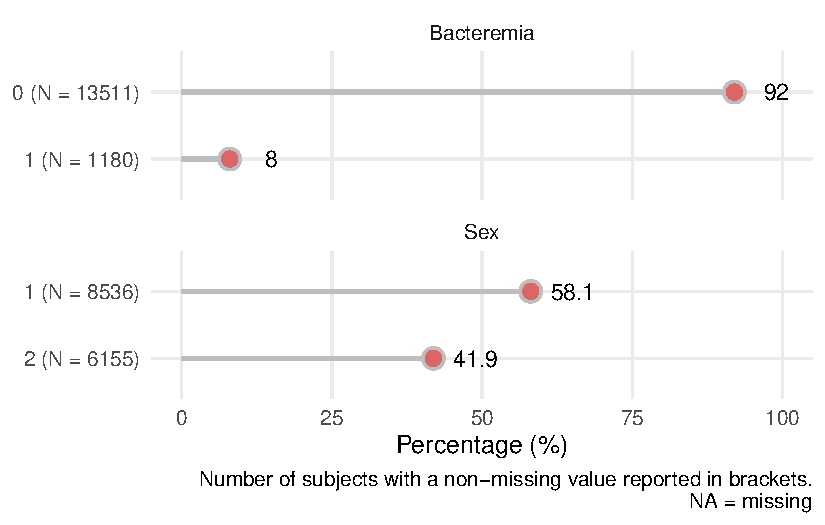
\includegraphics{./Bact_univar_files/figure-pdf/catplot-1.pdf}

\hypertarget{continuous-variables}{%
\section{Continuous variables}\label{continuous-variables}}

\hypertarget{u2-univariate-distributions-of-continuous-variables}{%
\subsection{U2: Univariate distributions of continuous
variables}\label{u2-univariate-distributions-of-continuous-variables}}

\hypertarget{u2-structural-variables}{%
\subsubsection{U2: Structural variables}\label{u2-structural-variables}}

The only structural continuous variables is AGE. This variable is also a
key predictor (see below).

\hypertarget{u2-key-predictors}{%
\subsubsection{U2: Key predictors}\label{u2-key-predictors}}

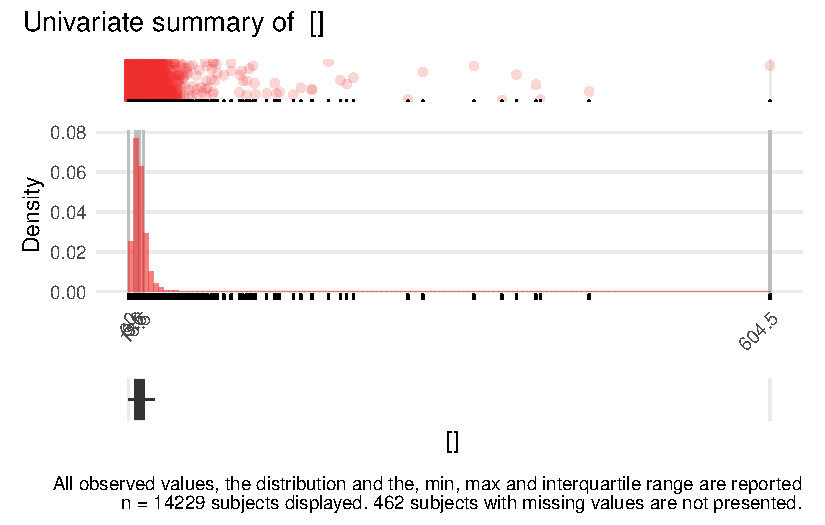
\includegraphics{./Bact_univar_files/figure-pdf/uni02-1.pdf}

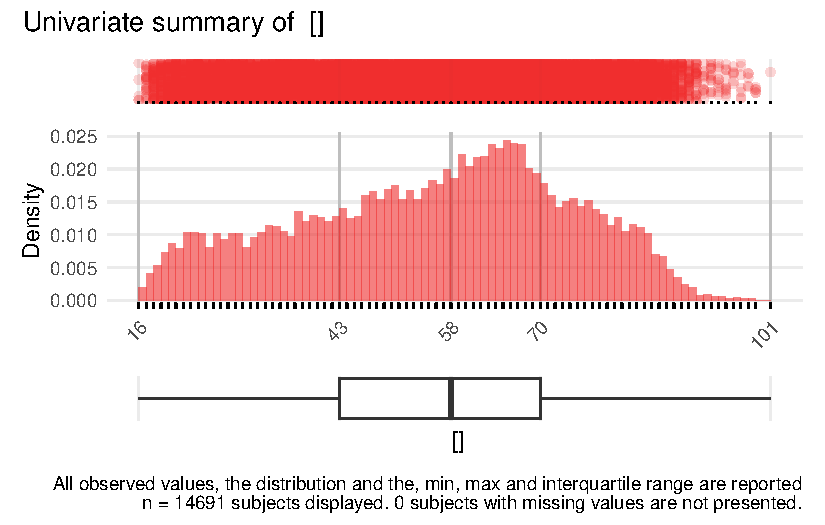
\includegraphics{./Bact_univar_files/figure-pdf/uni02-2.pdf}

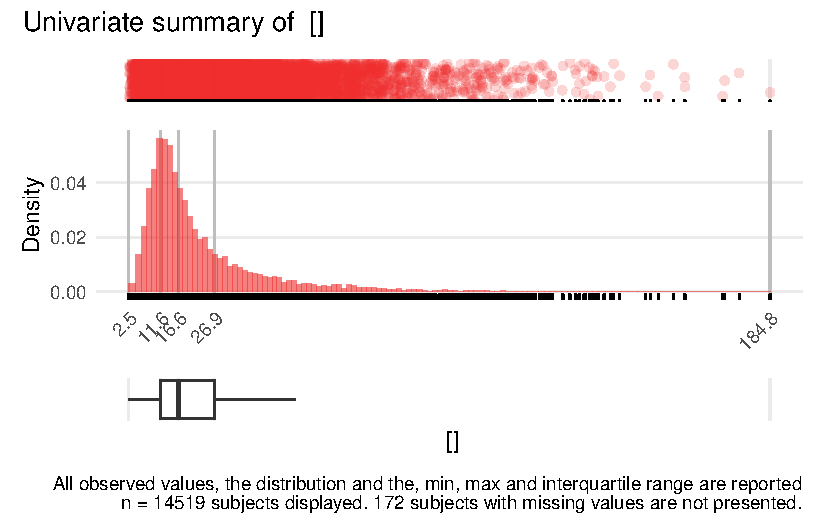
\includegraphics{./Bact_univar_files/figure-pdf/uni02-3.pdf}

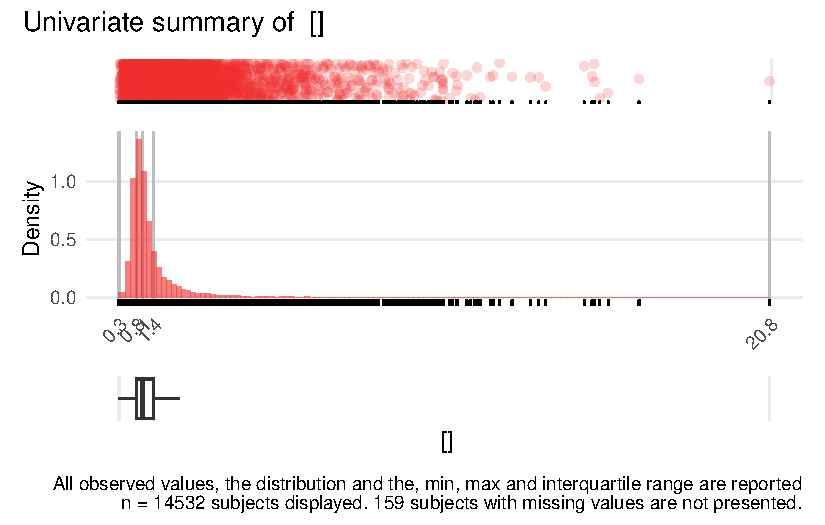
\includegraphics{./Bact_univar_files/figure-pdf/uni02-4.pdf}

\begin{verbatim}
Warning: Removed 1 rows containing missing values (geom_bar).
\end{verbatim}

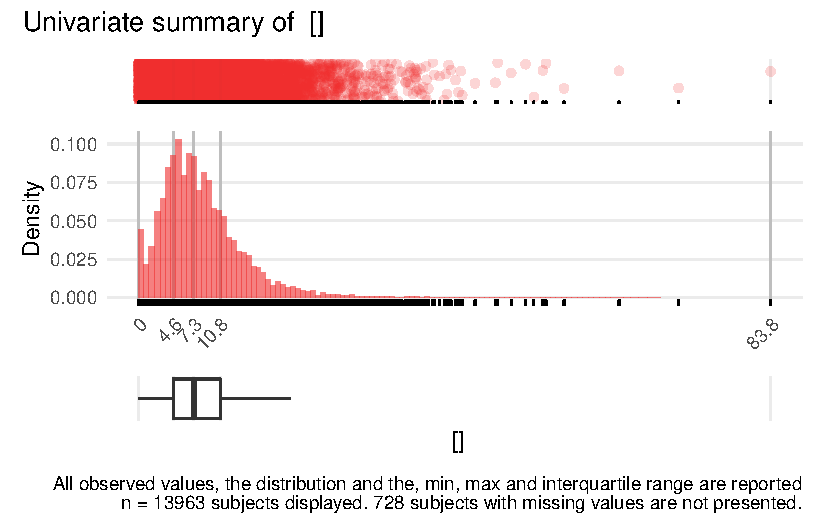
\includegraphics{./Bact_univar_files/figure-pdf/uni02-5.pdf}

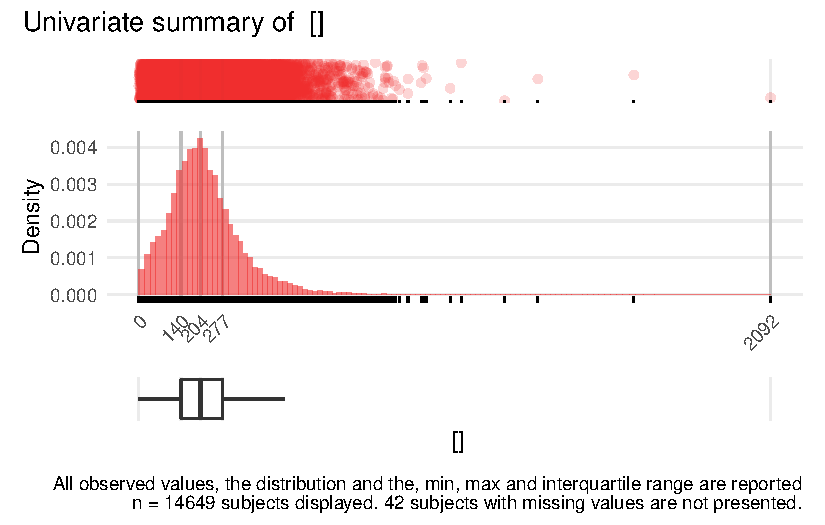
\includegraphics{./Bact_univar_files/figure-pdf/uni02-6.pdf}

\hypertarget{u2-predictors-of-medium-importance}{%
\subsubsection{U2: Predictors of medium
importance}\label{u2-predictors-of-medium-importance}}

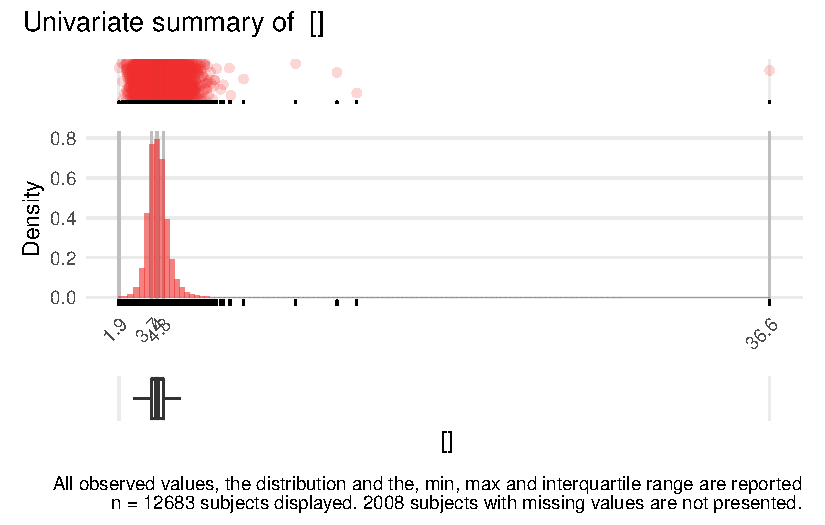
\includegraphics{./Bact_univar_files/figure-pdf/uni03-1.pdf}

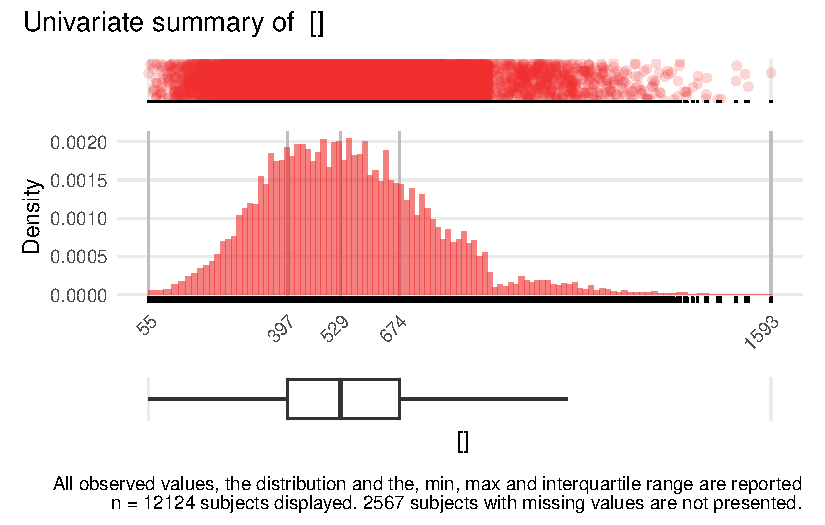
\includegraphics{./Bact_univar_files/figure-pdf/uni03-2.pdf}

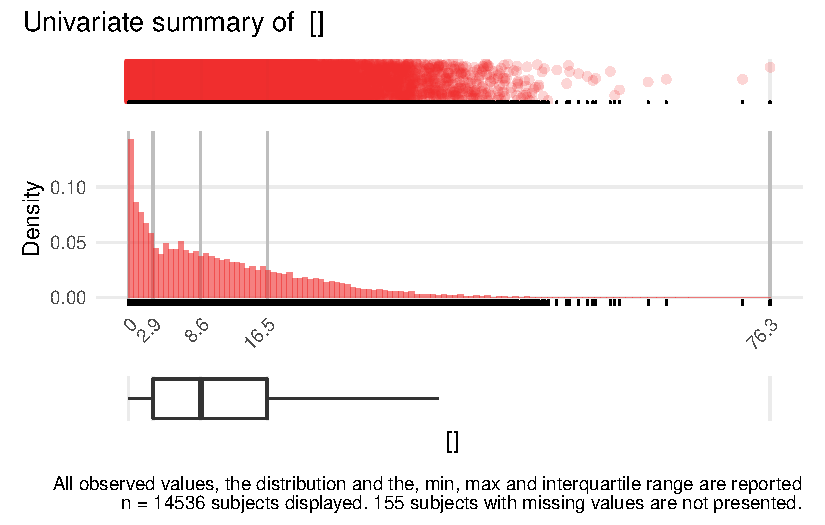
\includegraphics{./Bact_univar_files/figure-pdf/uni03-3.pdf}

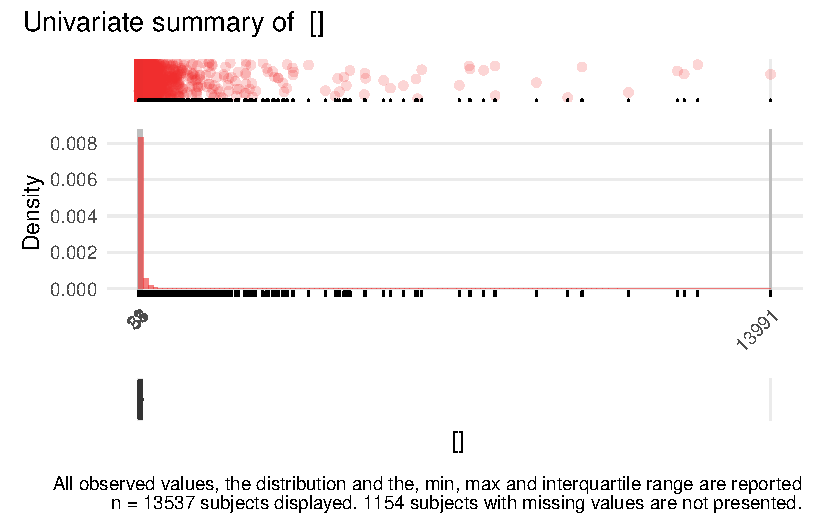
\includegraphics{./Bact_univar_files/figure-pdf/uni03-4.pdf}

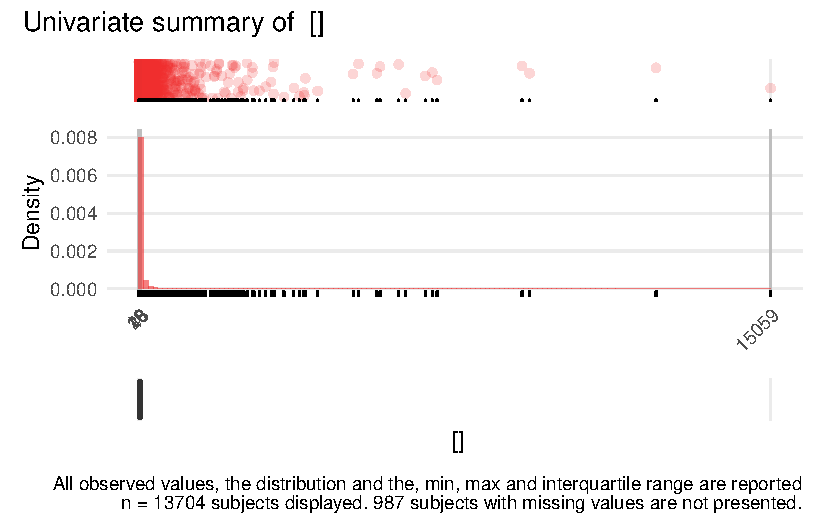
\includegraphics{./Bact_univar_files/figure-pdf/uni03-5.pdf}

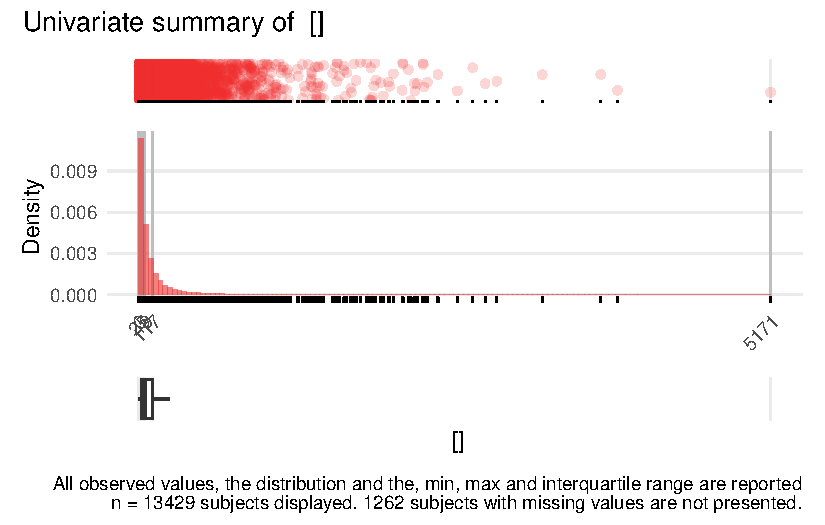
\includegraphics{./Bact_univar_files/figure-pdf/uni03-6.pdf}

\hypertarget{u2-remaining-predictors}{%
\subsubsection{U2: Remaining predictors}\label{u2-remaining-predictors}}

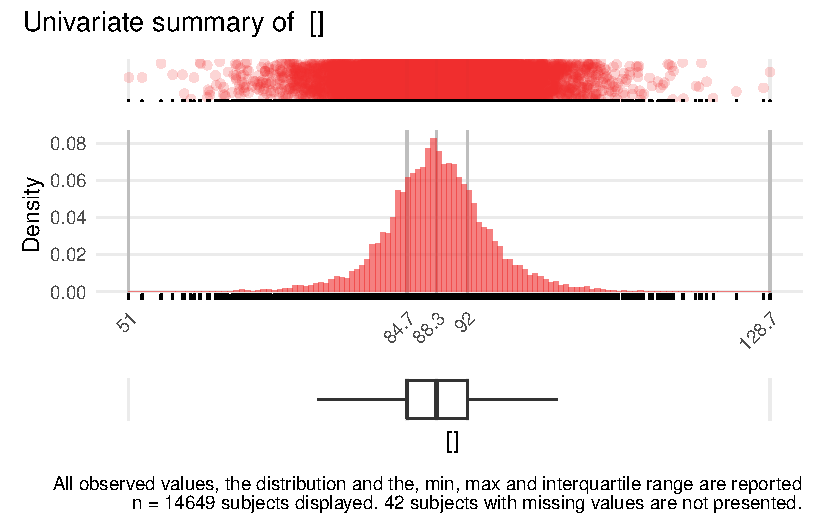
\includegraphics{./Bact_univar_files/figure-pdf/uni04-1.pdf}

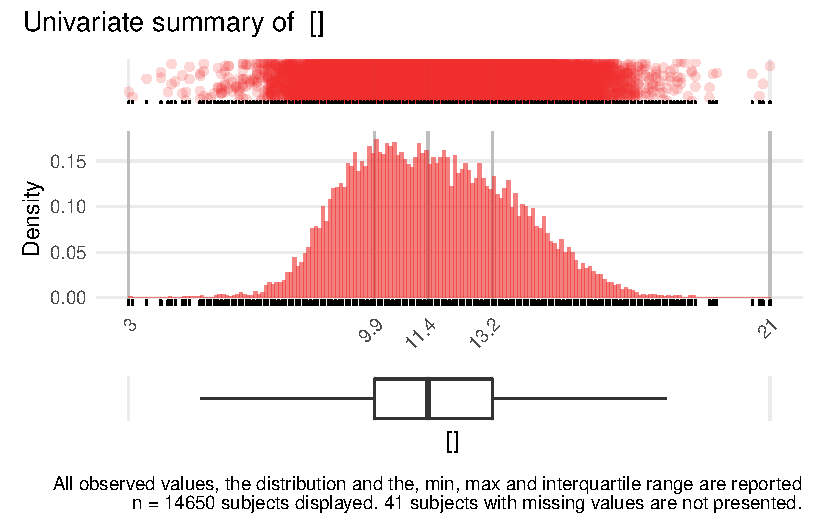
\includegraphics{./Bact_univar_files/figure-pdf/uni04-2.pdf}

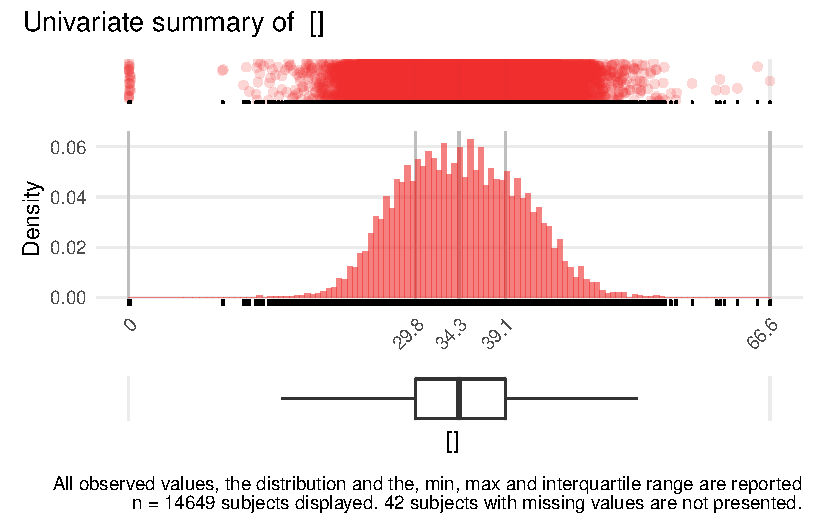
\includegraphics{./Bact_univar_files/figure-pdf/uni04-3.pdf}

\begin{verbatim}
Warning: Removed 1 rows containing missing values (geom_bar).
\end{verbatim}

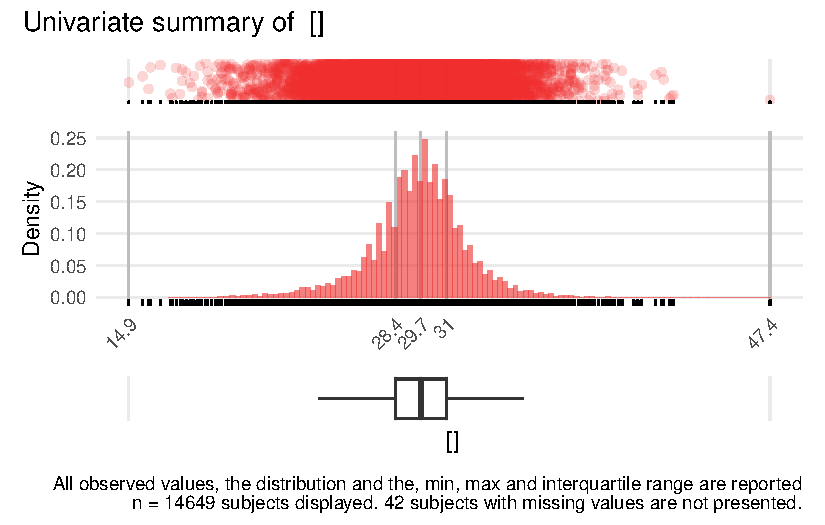
\includegraphics{./Bact_univar_files/figure-pdf/uni04-4.pdf}

\begin{verbatim}
Warning: Removed 1 rows containing missing values (geom_bar).
\end{verbatim}

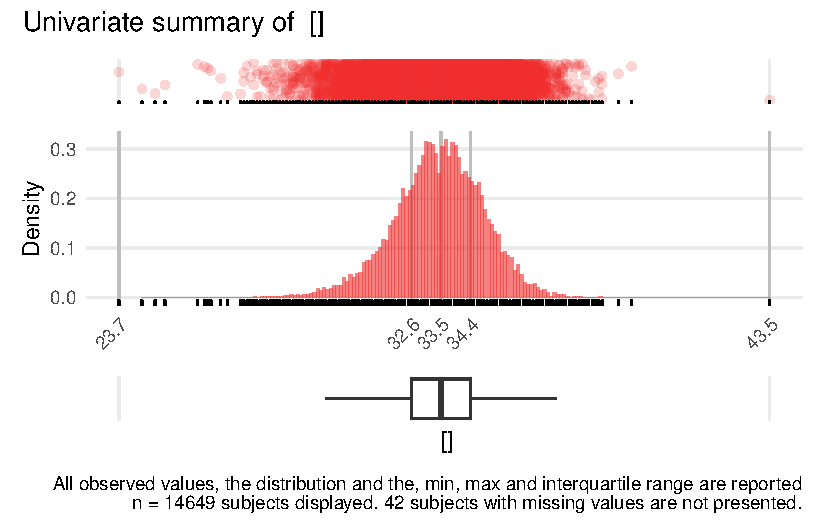
\includegraphics{./Bact_univar_files/figure-pdf/uni04-5.pdf}

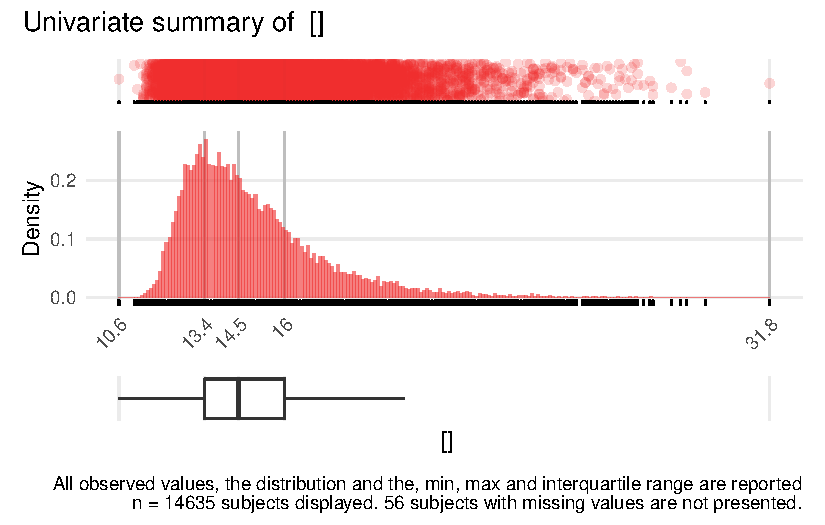
\includegraphics{./Bact_univar_files/figure-pdf/uni04-6.pdf}

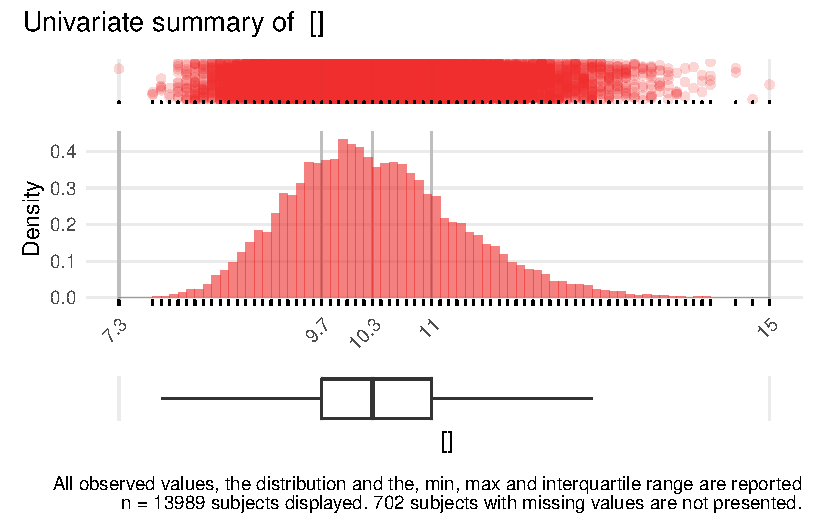
\includegraphics{./Bact_univar_files/figure-pdf/uni04-7.pdf}

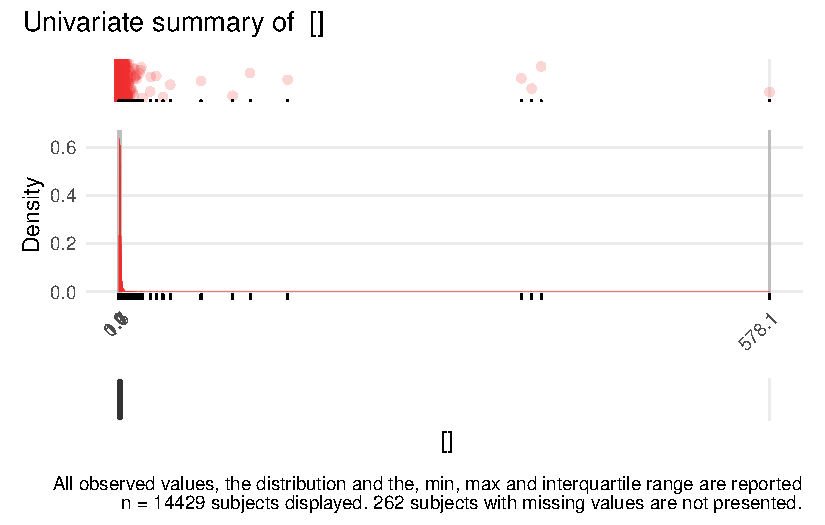
\includegraphics{./Bact_univar_files/figure-pdf/uni04-8.pdf}

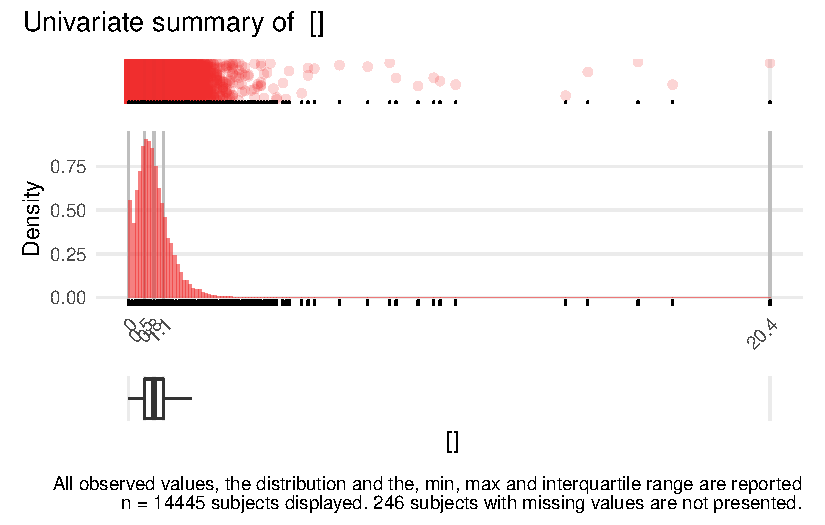
\includegraphics{./Bact_univar_files/figure-pdf/uni04-9.pdf}

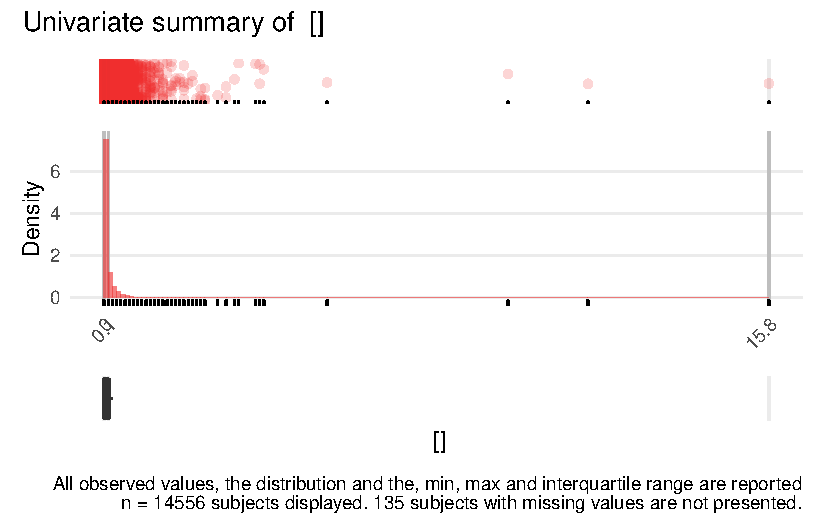
\includegraphics{./Bact_univar_files/figure-pdf/uni04-10.pdf}

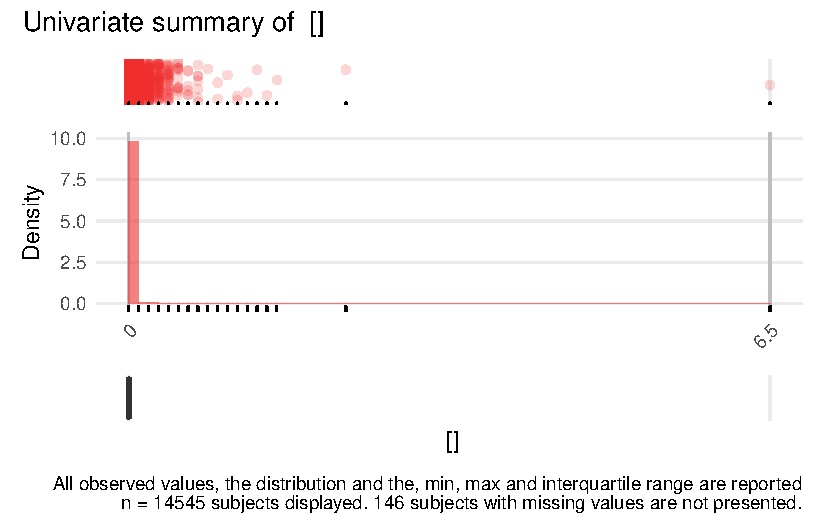
\includegraphics{./Bact_univar_files/figure-pdf/uni04-11.pdf}

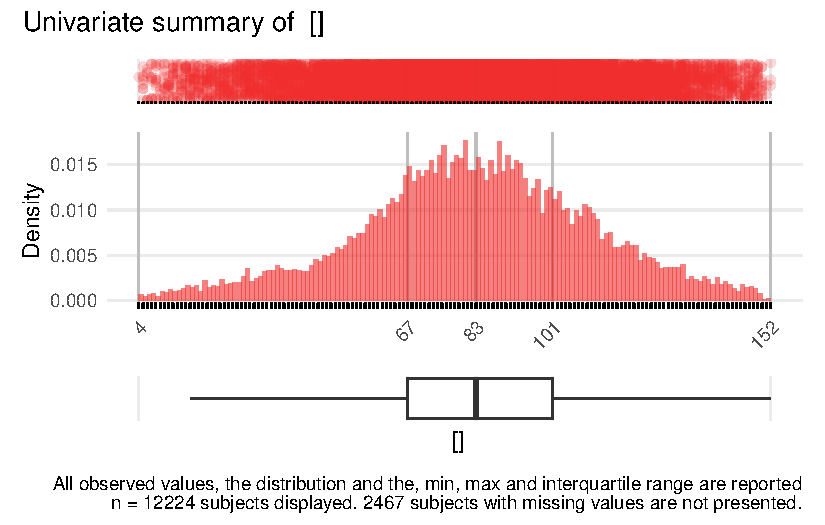
\includegraphics{./Bact_univar_files/figure-pdf/uni04-12.pdf}

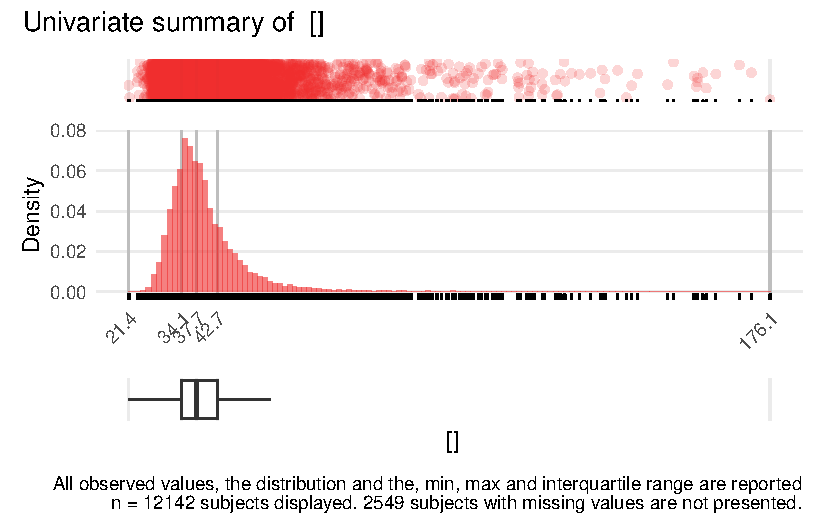
\includegraphics{./Bact_univar_files/figure-pdf/uni04-13.pdf}

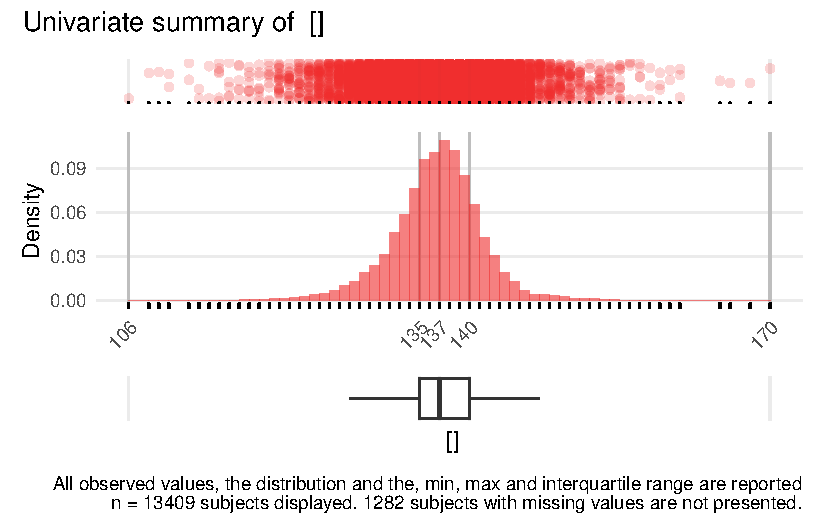
\includegraphics{./Bact_univar_files/figure-pdf/uni04-14.pdf}

\begin{verbatim}
Warning: Removed 1 rows containing missing values (geom_bar).
\end{verbatim}

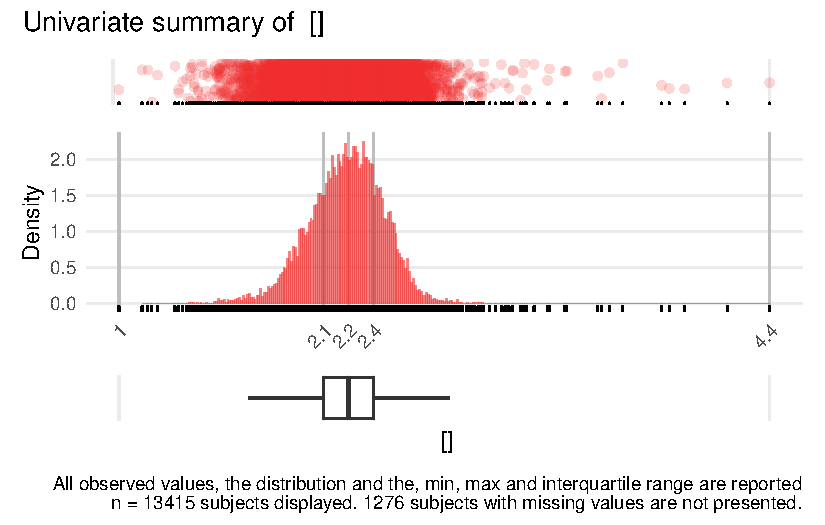
\includegraphics{./Bact_univar_files/figure-pdf/uni04-15.pdf}

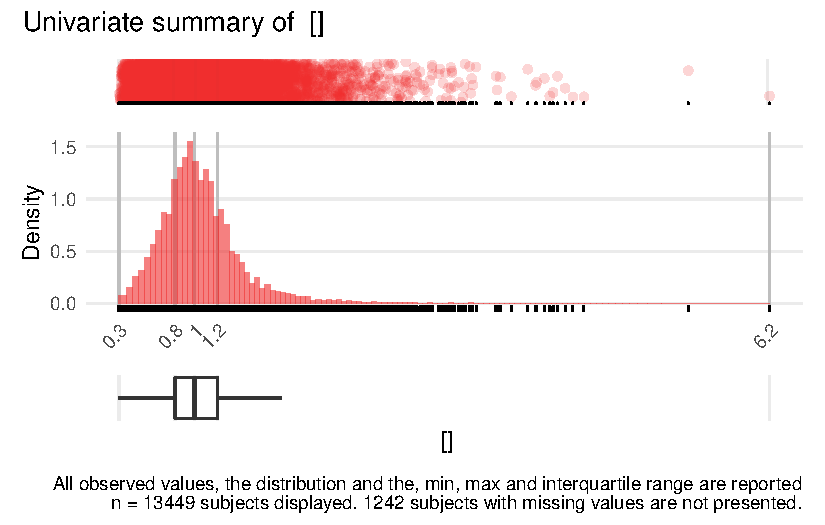
\includegraphics{./Bact_univar_files/figure-pdf/uni04-16.pdf}

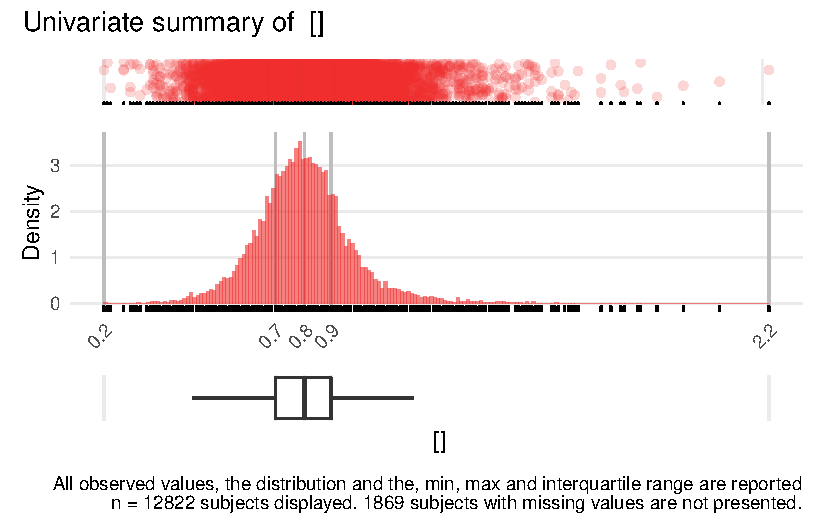
\includegraphics{./Bact_univar_files/figure-pdf/uni04-17.pdf}

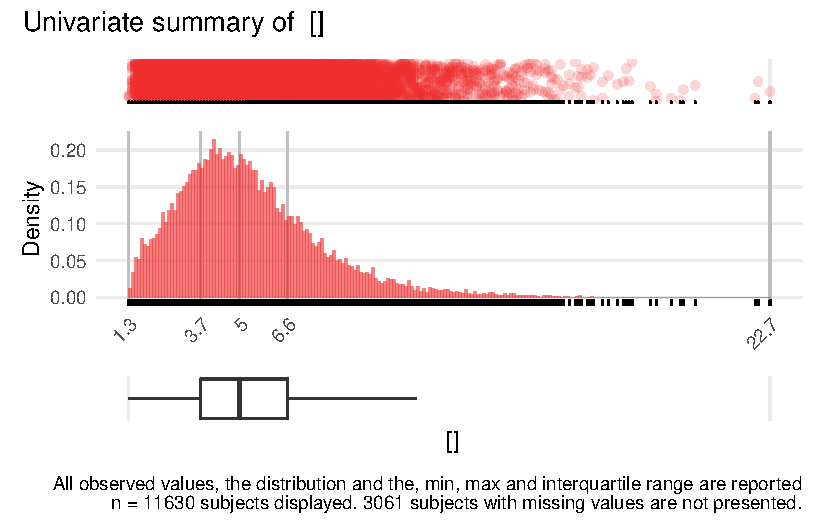
\includegraphics{./Bact_univar_files/figure-pdf/uni04-18.pdf}

\begin{verbatim}
Warning: Removed 1 rows containing missing values (geom_bar).
\end{verbatim}

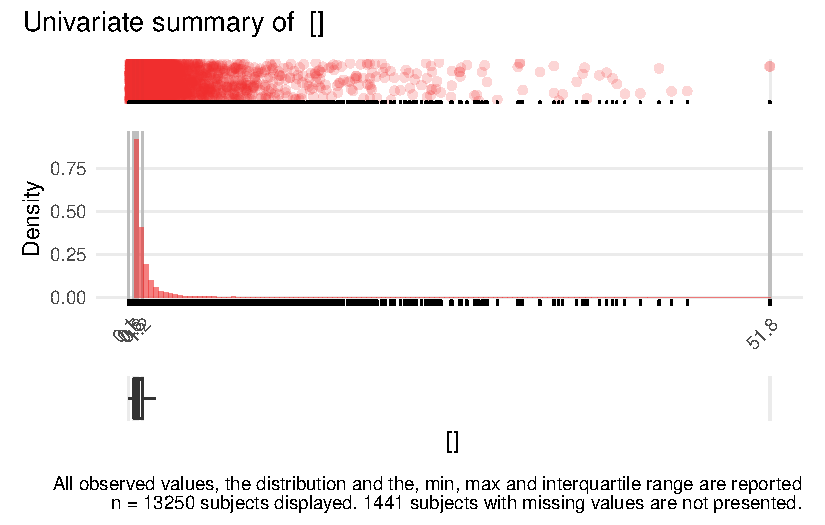
\includegraphics{./Bact_univar_files/figure-pdf/uni04-19.pdf}

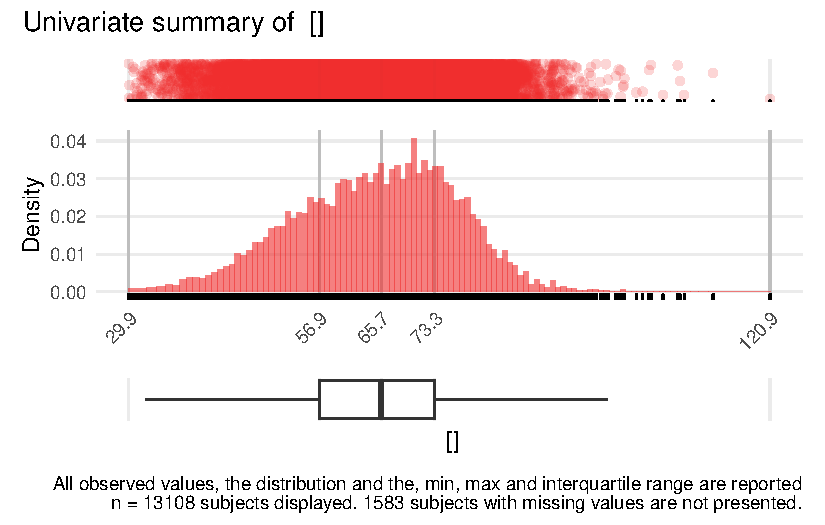
\includegraphics{./Bact_univar_files/figure-pdf/uni04-20.pdf}

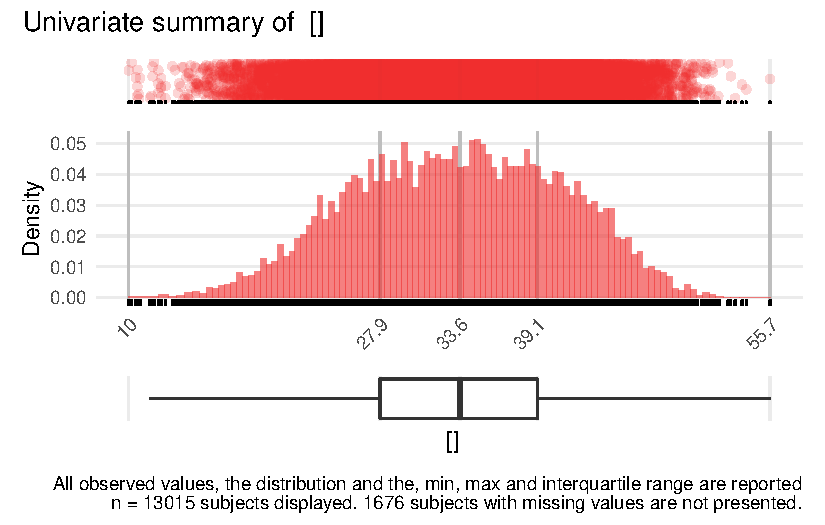
\includegraphics{./Bact_univar_files/figure-pdf/uni04-21.pdf}

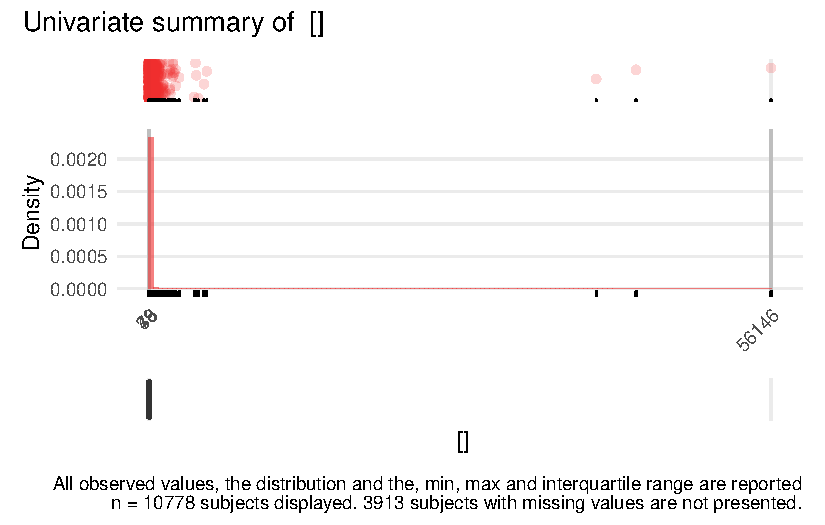
\includegraphics{./Bact_univar_files/figure-pdf/uni04-22.pdf}

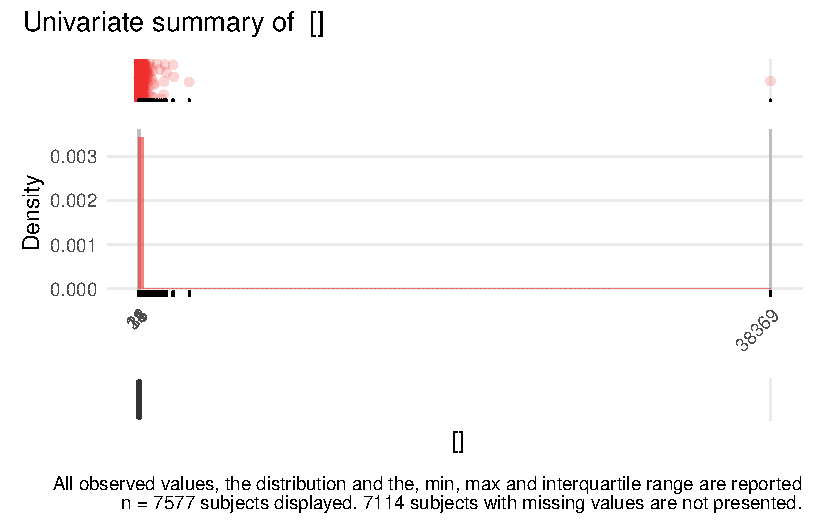
\includegraphics{./Bact_univar_files/figure-pdf/uni04-23.pdf}

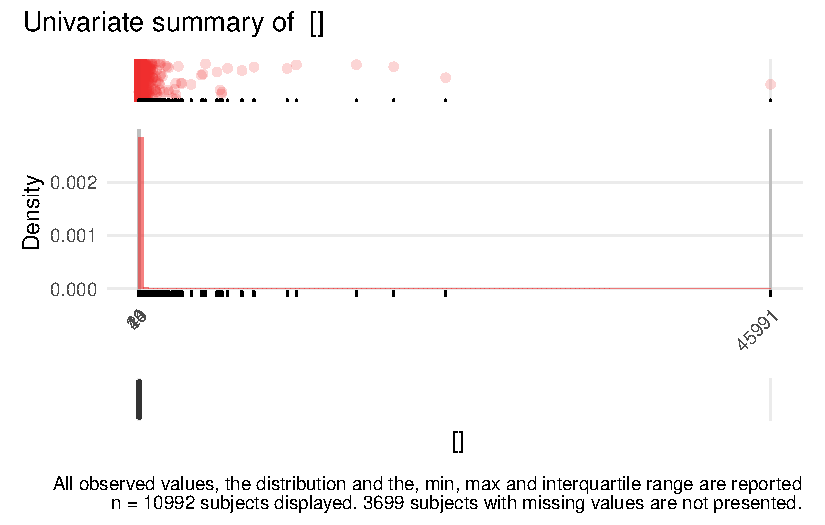
\includegraphics{./Bact_univar_files/figure-pdf/uni04-24.pdf}

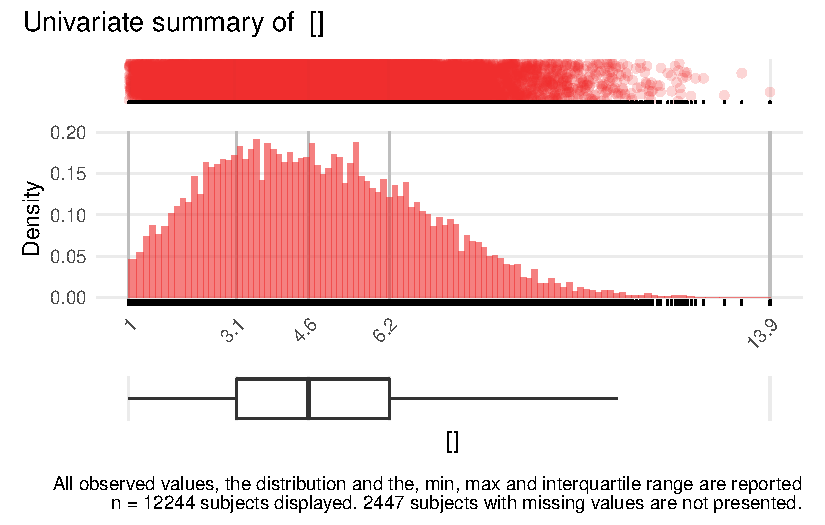
\includegraphics{./Bact_univar_files/figure-pdf/uni04-25.pdf}

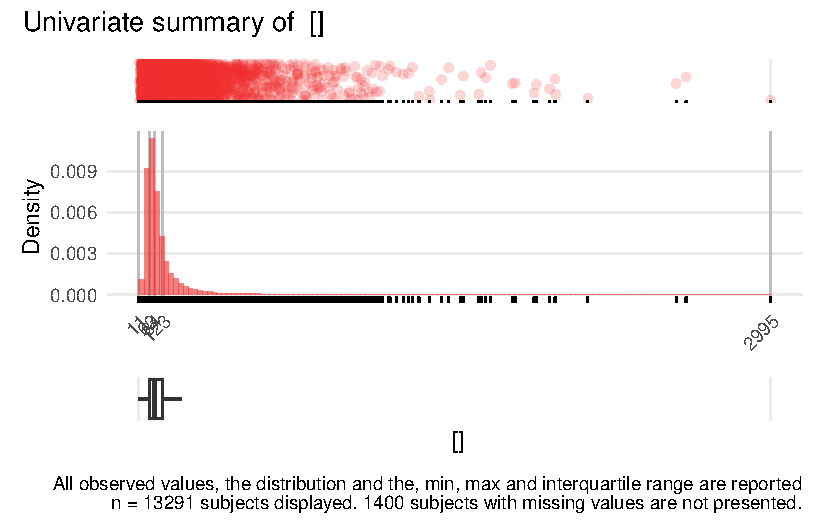
\includegraphics{./Bact_univar_files/figure-pdf/uni04-26.pdf}

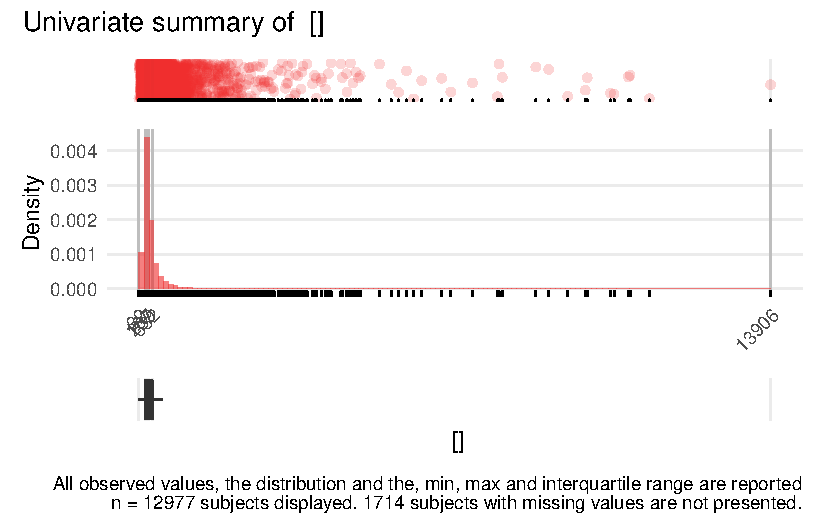
\includegraphics{./Bact_univar_files/figure-pdf/uni04-27.pdf}

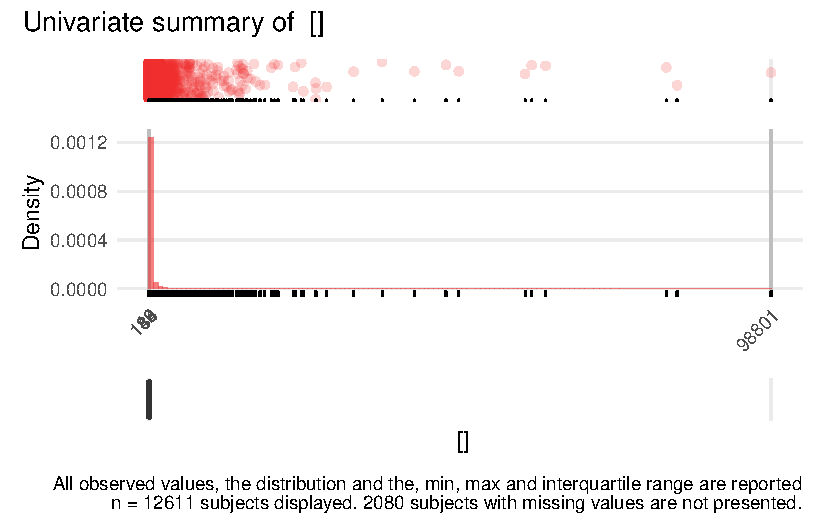
\includegraphics{./Bact_univar_files/figure-pdf/uni04-28.pdf}

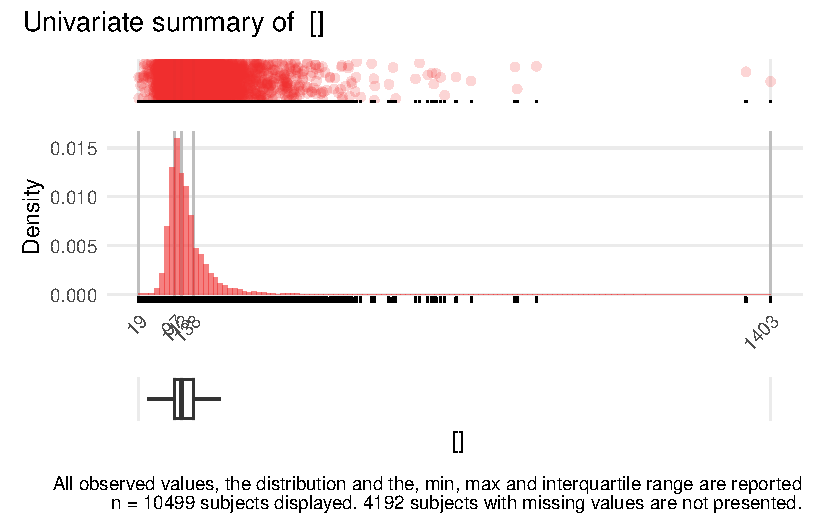
\includegraphics{./Bact_univar_files/figure-pdf/uni04-29.pdf}

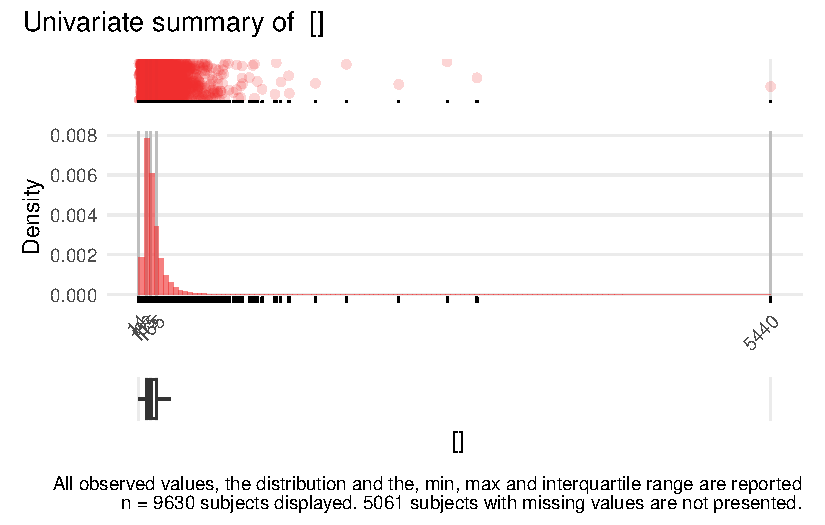
\includegraphics{./Bact_univar_files/figure-pdf/uni04-30.pdf}

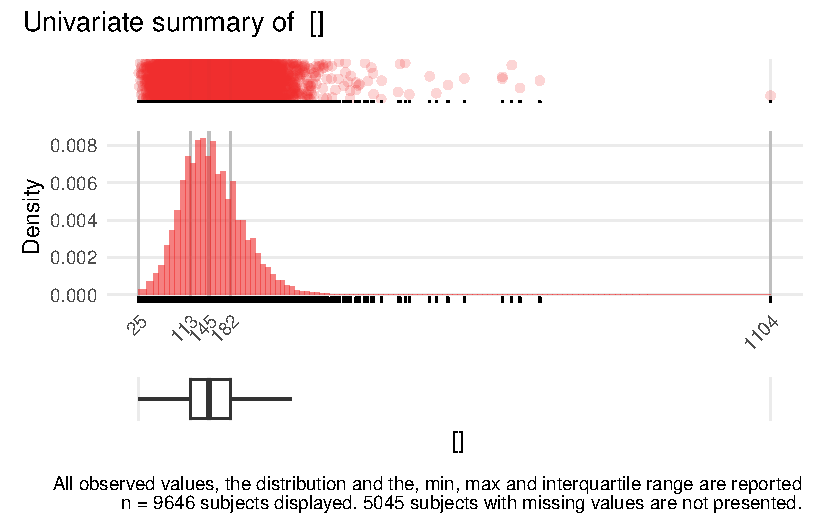
\includegraphics{./Bact_univar_files/figure-pdf/uni04-31.pdf}

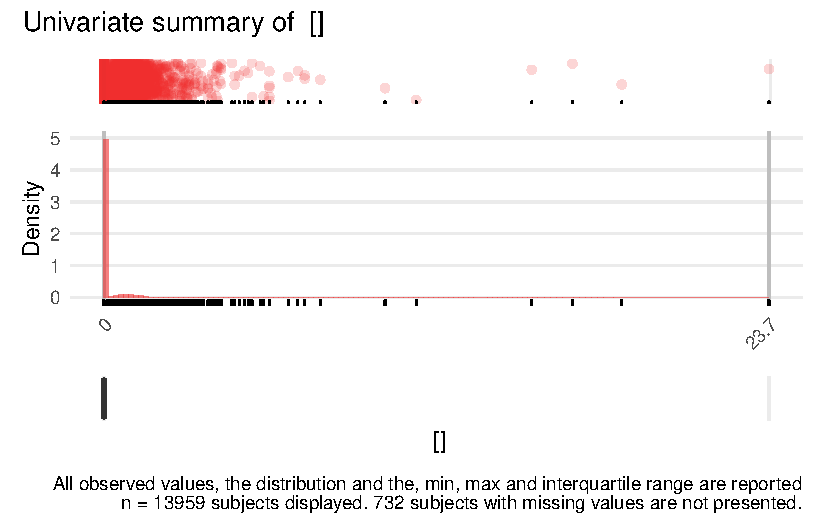
\includegraphics{./Bact_univar_files/figure-pdf/uni04-32.pdf}

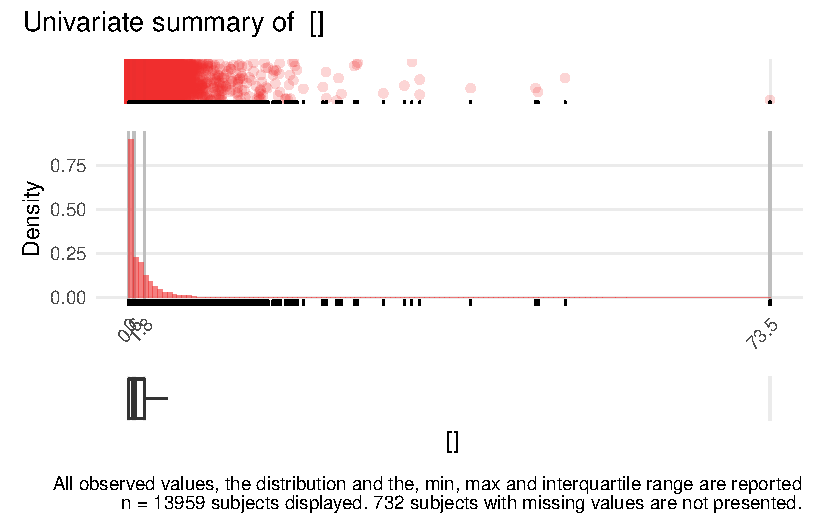
\includegraphics{./Bact_univar_files/figure-pdf/uni04-33.pdf}

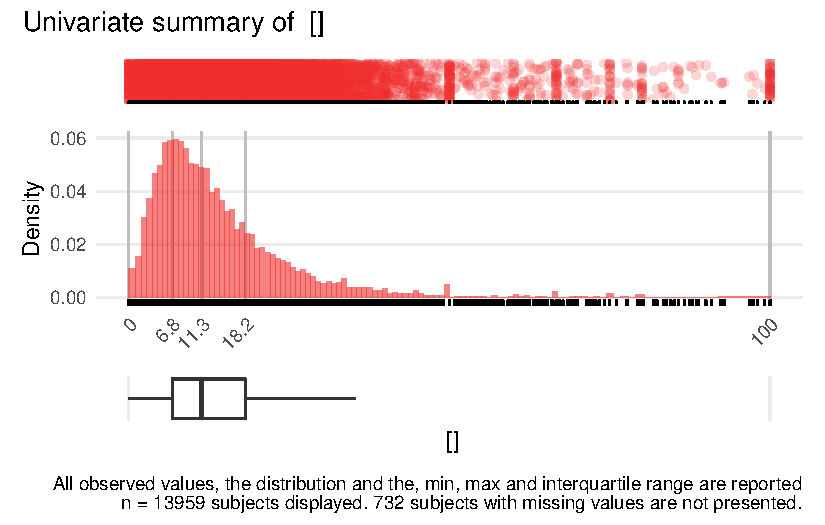
\includegraphics{./Bact_univar_files/figure-pdf/uni04-34.pdf}

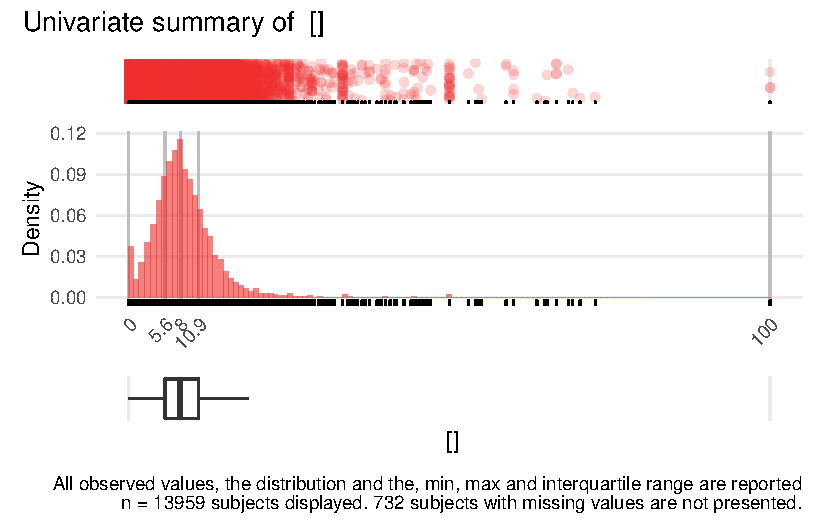
\includegraphics{./Bact_univar_files/figure-pdf/uni04-35.pdf}

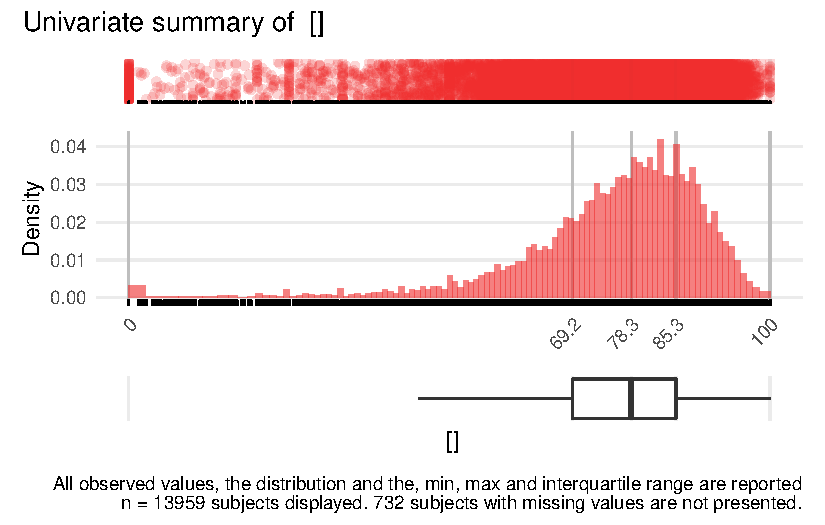
\includegraphics{./Bact_univar_files/figure-pdf/uni04-36.pdf}

\includegraphics{./Bact_univar_files/figure-pdf/uni04-37.pdf}

\includegraphics{./Bact_univar_files/figure-pdf/uni04-38.pdf}

\hypertarget{numerical-summaries}{%
\subsection{Numerical summaries}\label{numerical-summaries}}

\hypertarget{key-predictors}{%
\subsubsection{Key predictors}\label{key-predictors}}

\begin{longtable}[]{@{}ll@{}}
\caption{Data summary}\tabularnewline
\toprule()
\endhead
Name & Piped data \\
Number of rows & 14691 \\
Number of columns & 6 \\
\_\_\_\_\_\_\_\_\_\_\_\_\_\_\_\_\_\_\_\_\_\_\_ & \\
Column type frequency: & \\
numeric & 6 \\
\_\_\_\_\_\_\_\_\_\_\_\_\_\_\_\_\_\_\_\_\_\_\_\_ & \\
Group variables & None \\
\bottomrule()
\end{longtable}

\textbf{Variable type: numeric}

\begin{longtable}[]{@{}
  >{\raggedright\arraybackslash}p{(\columnwidth - 20\tabcolsep) * \real{0.1102}}
  >{\raggedleft\arraybackslash}p{(\columnwidth - 20\tabcolsep) * \real{0.0787}}
  >{\raggedleft\arraybackslash}p{(\columnwidth - 20\tabcolsep) * \real{0.1102}}
  >{\raggedleft\arraybackslash}p{(\columnwidth - 20\tabcolsep) * \real{0.0551}}
  >{\raggedleft\arraybackslash}p{(\columnwidth - 20\tabcolsep) * \real{0.0551}}
  >{\raggedleft\arraybackslash}p{(\columnwidth - 20\tabcolsep) * \real{0.0472}}
  >{\raggedleft\arraybackslash}p{(\columnwidth - 20\tabcolsep) * \real{0.0551}}
  >{\raggedleft\arraybackslash}p{(\columnwidth - 20\tabcolsep) * \real{0.0472}}
  >{\raggedleft\arraybackslash}p{(\columnwidth - 20\tabcolsep) * \real{0.0551}}
  >{\raggedleft\arraybackslash}p{(\columnwidth - 20\tabcolsep) * \real{0.0630}}
  >{\raggedright\arraybackslash}p{(\columnwidth - 20\tabcolsep) * \real{0.3228}}@{}}
\toprule()
\begin{minipage}[b]{\linewidth}\raggedright
skim\_variable
\end{minipage} & \begin{minipage}[b]{\linewidth}\raggedleft
n\_missing
\end{minipage} & \begin{minipage}[b]{\linewidth}\raggedleft
complete\_rate
\end{minipage} & \begin{minipage}[b]{\linewidth}\raggedleft
mean
\end{minipage} & \begin{minipage}[b]{\linewidth}\raggedleft
sd
\end{minipage} & \begin{minipage}[b]{\linewidth}\raggedleft
p0
\end{minipage} & \begin{minipage}[b]{\linewidth}\raggedleft
p25
\end{minipage} & \begin{minipage}[b]{\linewidth}\raggedleft
p50
\end{minipage} & \begin{minipage}[b]{\linewidth}\raggedleft
p75
\end{minipage} & \begin{minipage}[b]{\linewidth}\raggedleft
p100
\end{minipage} & \begin{minipage}[b]{\linewidth}\raggedright
hist
\end{minipage} \\
\midrule()
\endhead
WBC & 462 & 0.97 & 11.23 & 12.92 & 0.00 & 6.63 & 9.6 & 13.53 & 604.47 &
▇▁▁▁▁ \\
AGE & 0 & 1.00 & 56.17 & 18.15 & 16.00 & 43.00 & 58.0 & 70.00 & 101.00 &
▃▅▇▆▁ \\
BUN & 172 & 0.99 & 22.66 & 18.11 & 2.50 & 11.60 & 16.6 & 26.90 & 184.80
& ▇▁▁▁▁ \\
CREA & 159 & 0.99 & 1.33 & 1.17 & 0.26 & 0.81 & 1.0 & 1.35 & 20.75 &
▇▁▁▁▁ \\
NEU & 728 & 0.95 & 8.37 & 5.61 & 0.00 & 4.60 & 7.3 & 10.80 & 83.80 &
▇▁▁▁▁ \\
PLT & 42 & 1.00 & 220.03 & 122.84 & 0.00 & 140.00 & 204.0 & 277.00 &
2092.00 & ▇▁▁▁▁ \\
\bottomrule()
\end{longtable}

\hypertarget{predictors-of-medium-importance}{%
\subsubsection{Predictors of medium
importance}\label{predictors-of-medium-importance}}

\begin{longtable}[]{@{}ll@{}}
\caption{Data summary}\tabularnewline
\toprule()
\endhead
Name & Piped data \\
Number of rows & 14691 \\
Number of columns & 6 \\
\_\_\_\_\_\_\_\_\_\_\_\_\_\_\_\_\_\_\_\_\_\_\_ & \\
Column type frequency: & \\
numeric & 6 \\
\_\_\_\_\_\_\_\_\_\_\_\_\_\_\_\_\_\_\_\_\_\_\_\_ & \\
Group variables & None \\
\bottomrule()
\end{longtable}

\textbf{Variable type: numeric}

\begin{longtable}[]{@{}
  >{\raggedright\arraybackslash}p{(\columnwidth - 20\tabcolsep) * \real{0.1085}}
  >{\raggedleft\arraybackslash}p{(\columnwidth - 20\tabcolsep) * \real{0.0775}}
  >{\raggedleft\arraybackslash}p{(\columnwidth - 20\tabcolsep) * \real{0.1085}}
  >{\raggedleft\arraybackslash}p{(\columnwidth - 20\tabcolsep) * \real{0.0543}}
  >{\raggedleft\arraybackslash}p{(\columnwidth - 20\tabcolsep) * \real{0.0543}}
  >{\raggedleft\arraybackslash}p{(\columnwidth - 20\tabcolsep) * \real{0.0465}}
  >{\raggedleft\arraybackslash}p{(\columnwidth - 20\tabcolsep) * \real{0.0543}}
  >{\raggedleft\arraybackslash}p{(\columnwidth - 20\tabcolsep) * \real{0.0543}}
  >{\raggedleft\arraybackslash}p{(\columnwidth - 20\tabcolsep) * \real{0.0543}}
  >{\raggedleft\arraybackslash}p{(\columnwidth - 20\tabcolsep) * \real{0.0698}}
  >{\raggedright\arraybackslash}p{(\columnwidth - 20\tabcolsep) * \real{0.3178}}@{}}
\toprule()
\begin{minipage}[b]{\linewidth}\raggedright
skim\_variable
\end{minipage} & \begin{minipage}[b]{\linewidth}\raggedleft
n\_missing
\end{minipage} & \begin{minipage}[b]{\linewidth}\raggedleft
complete\_rate
\end{minipage} & \begin{minipage}[b]{\linewidth}\raggedleft
mean
\end{minipage} & \begin{minipage}[b]{\linewidth}\raggedleft
sd
\end{minipage} & \begin{minipage}[b]{\linewidth}\raggedleft
p0
\end{minipage} & \begin{minipage}[b]{\linewidth}\raggedleft
p25
\end{minipage} & \begin{minipage}[b]{\linewidth}\raggedleft
p50
\end{minipage} & \begin{minipage}[b]{\linewidth}\raggedleft
p75
\end{minipage} & \begin{minipage}[b]{\linewidth}\raggedleft
p100
\end{minipage} & \begin{minipage}[b]{\linewidth}\raggedright
hist
\end{minipage} \\
\midrule()
\endhead
POTASS & 2008 & 0.86 & 4.00 & 0.64 & 1.92 & 3.66 & 3.95 & 4.29 & 36.62 &
▇▁▁▁▁ \\
FIB & 2567 & 0.83 & 547.36 & 208.13 & 55.00 & 397.00 & 529.00 & 674.00 &
1593.00 & ▃▇▃▁▁ \\
CRP & 155 & 0.99 & 10.92 & 9.58 & 0.00 & 2.87 & 8.57 & 16.45 & 76.32 &
▇▂▁▁▁ \\
ASAT & 1154 & 0.92 & 86.90 & 404.69 & 3.00 & 22.00 & 31.00 & 56.00 &
13991.00 & ▇▁▁▁▁ \\
ALAT & 987 & 0.93 & 67.66 & 311.05 & 0.00 & 16.00 & 26.00 & 48.00 &
15059.00 & ▇▁▁▁▁ \\
GGT & 1262 & 0.91 & 115.06 & 208.98 & 3.00 & 25.00 & 49.00 & 117.00 &
5171.00 & ▇▁▁▁▁ \\
\bottomrule()
\end{longtable}

\hypertarget{remaining-predictors}{%
\subsubsection{Remaining predictors}\label{remaining-predictors}}

\begin{longtable}[]{@{}ll@{}}
\caption{Data summary}\tabularnewline
\toprule()
\endhead
Name & Piped data \\
Number of rows & 14691 \\
Number of columns & 38 \\
\_\_\_\_\_\_\_\_\_\_\_\_\_\_\_\_\_\_\_\_\_\_\_ & \\
Column type frequency: & \\
numeric & 38 \\
\_\_\_\_\_\_\_\_\_\_\_\_\_\_\_\_\_\_\_\_\_\_\_\_ & \\
Group variables & None \\
\bottomrule()
\end{longtable}

\textbf{Variable type: numeric}

\begin{longtable}[]{@{}
  >{\raggedright\arraybackslash}p{(\columnwidth - 20\tabcolsep) * \real{0.1069}}
  >{\raggedleft\arraybackslash}p{(\columnwidth - 20\tabcolsep) * \real{0.0763}}
  >{\raggedleft\arraybackslash}p{(\columnwidth - 20\tabcolsep) * \real{0.1069}}
  >{\raggedleft\arraybackslash}p{(\columnwidth - 20\tabcolsep) * \real{0.0534}}
  >{\raggedleft\arraybackslash}p{(\columnwidth - 20\tabcolsep) * \real{0.0611}}
  >{\raggedleft\arraybackslash}p{(\columnwidth - 20\tabcolsep) * \real{0.0534}}
  >{\raggedleft\arraybackslash}p{(\columnwidth - 20\tabcolsep) * \real{0.0534}}
  >{\raggedleft\arraybackslash}p{(\columnwidth - 20\tabcolsep) * \real{0.0534}}
  >{\raggedleft\arraybackslash}p{(\columnwidth - 20\tabcolsep) * \real{0.0534}}
  >{\raggedleft\arraybackslash}p{(\columnwidth - 20\tabcolsep) * \real{0.0687}}
  >{\raggedright\arraybackslash}p{(\columnwidth - 20\tabcolsep) * \real{0.3130}}@{}}
\toprule()
\begin{minipage}[b]{\linewidth}\raggedright
skim\_variable
\end{minipage} & \begin{minipage}[b]{\linewidth}\raggedleft
n\_missing
\end{minipage} & \begin{minipage}[b]{\linewidth}\raggedleft
complete\_rate
\end{minipage} & \begin{minipage}[b]{\linewidth}\raggedleft
mean
\end{minipage} & \begin{minipage}[b]{\linewidth}\raggedleft
sd
\end{minipage} & \begin{minipage}[b]{\linewidth}\raggedleft
p0
\end{minipage} & \begin{minipage}[b]{\linewidth}\raggedleft
p25
\end{minipage} & \begin{minipage}[b]{\linewidth}\raggedleft
p50
\end{minipage} & \begin{minipage}[b]{\linewidth}\raggedleft
p75
\end{minipage} & \begin{minipage}[b]{\linewidth}\raggedleft
p100
\end{minipage} & \begin{minipage}[b]{\linewidth}\raggedright
hist
\end{minipage} \\
\midrule()
\endhead
MCV & 42 & 1.00 & 88.35 & 6.46 & 51.00 & 84.70 & 88.30 & 92.00 & 128.70
& ▁▁▇▁▁ \\
HGB & 41 & 1.00 & 11.57 & 2.25 & 3.00 & 9.90 & 11.40 & 13.20 & 21.00 &
▁▅▇▂▁ \\
HCT & 42 & 1.00 & 34.48 & 6.51 & 0.00 & 29.80 & 34.30 & 39.10 & 66.60 &
▁▁▇▂▁ \\
MCH & 42 & 1.00 & 29.58 & 2.53 & 14.90 & 28.40 & 29.70 & 31.00 & 47.40 &
▁▂▇▁▁ \\
MCHC & 42 & 1.00 & 33.47 & 1.40 & 23.70 & 32.60 & 33.50 & 34.40 & 43.50
& ▁▁▇▁▁ \\
RDW & 56 & 1.00 & 15.00 & 2.29 & 10.60 & 13.40 & 14.50 & 16.00 & 31.80 &
▇▅▁▁▁ \\
MPV & 702 & 0.95 & 10.38 & 1.01 & 7.30 & 9.70 & 10.30 & 11.00 & 15.00 &
▁▇▇▁▁ \\
LYM & 262 & 0.98 & 1.37 & 7.46 & 0.00 & 0.70 & 1.00 & 1.60 & 578.10 &
▇▁▁▁▁ \\
MONO & 246 & 0.98 & 0.85 & 0.65 & 0.00 & 0.50 & 0.80 & 1.10 & 20.40 &
▇▁▁▁▁ \\
EOS & 135 & 0.99 & 0.11 & 0.27 & 0.00 & 0.00 & 0.10 & 0.10 & 15.80 &
▇▁▁▁▁ \\
BASO & 146 & 0.99 & 0.02 & 0.08 & 0.00 & 0.00 & 0.00 & 0.00 & 6.50 &
▇▁▁▁▁ \\
NT & 2467 & 0.83 & 83.22 & 27.15 & 4.00 & 67.00 & 83.00 & 101.00 &
152.00 & ▁▃▇▆▂ \\
APTT & 2549 & 0.83 & 40.06 & 10.97 & 21.40 & 34.10 & 37.70 & 42.70 &
176.10 & ▇▁▁▁▁ \\
SODIUM & 1282 & 0.91 & 137.21 & 4.73 & 106.00 & 135.00 & 137.00 & 140.00
& 170.00 & ▁▁▇▁▁ \\
CA & 1276 & 0.91 & 2.21 & 0.20 & 1.03 & 2.09 & 2.22 & 2.35 & 4.40 &
▁▇▂▁▁ \\
PHOS & 1242 & 0.92 & 1.05 & 0.40 & 0.30 & 0.81 & 0.99 & 1.20 & 6.22 &
▇▁▁▁▁ \\
MG & 1869 & 0.87 & 0.81 & 0.15 & 0.20 & 0.72 & 0.81 & 0.89 & 2.22 &
▁▇▁▁▁ \\
HS & 3061 & 0.79 & 5.41 & 2.45 & 1.30 & 3.70 & 5.00 & 6.60 & 22.70 &
▇▅▁▁▁ \\
GBIL & 1441 & 0.90 & 1.41 & 2.75 & 0.11 & 0.53 & 0.77 & 1.23 & 51.77 &
▇▁▁▁▁ \\
TP & 1583 & 0.89 & 64.90 & 11.46 & 29.90 & 56.90 & 65.70 & 73.30 &
120.90 & ▂▇▇▁▁ \\
ALB & 1676 & 0.89 & 33.42 & 7.44 & 10.00 & 27.90 & 33.60 & 39.10 & 55.70
& ▁▅▇▆▁ \\
AMY & 3913 & 0.73 & 90.83 & 805.23 & 8.00 & 33.00 & 49.00 & 76.00 &
56146.00 & ▇▁▁▁▁ \\
PAMY & 7114 & 0.52 & 41.66 & 448.01 & 1.00 & 14.00 & 22.00 & 36.00 &
38369.00 & ▇▁▁▁▁ \\
LIP & 3699 & 0.75 & 63.82 & 603.89 & 0.00 & 14.00 & 23.00 & 40.00 &
45991.00 & ▇▁▁▁▁ \\
CHE & 2447 & 0.83 & 4.79 & 2.10 & 0.98 & 3.15 & 4.60 & 6.22 & 13.89 &
▆▇▅▁▁ \\
AP & 1400 & 0.90 & 118.78 & 132.87 & 11.00 & 63.00 & 84.00 & 123.00 &
2995.00 & ▇▁▁▁▁ \\
LDH & 1714 & 0.88 & 331.15 & 475.23 & 39.00 & 187.00 & 239.00 & 332.00 &
13906.00 & ▇▁▁▁▁ \\
CK & 2080 & 0.86 & 385.01 & 2241.21 & 8.00 & 42.00 & 80.00 & 184.00 &
98801.00 & ▇▁▁▁▁ \\
GLU & 4192 & 0.71 & 126.41 & 56.91 & 19.00 & 97.00 & 113.00 & 138.00 &
1403.00 & ▇▁▁▁▁ \\
TRIG & 5061 & 0.66 & 141.71 & 120.69 & 14.00 & 83.00 & 115.00 & 165.00 &
5440.00 & ▇▁▁▁▁ \\
CHOL & 5045 & 0.66 & 150.80 & 55.51 & 25.00 & 113.00 & 145.00 & 182.00 &
1104.00 & ▇▁▁▁▁ \\
BASOR & 732 & 0.95 & 0.15 & 0.59 & 0.00 & 0.00 & 0.00 & 0.00 & 23.66 &
▇▁▁▁▁ \\
EOSR & 732 & 0.95 & 1.30 & 2.36 & 0.00 & 0.00 & 0.59 & 1.79 & 73.49 &
▇▁▁▁▁ \\
LYMR & 732 & 0.95 & 14.61 & 12.74 & 0.00 & 6.76 & 11.34 & 18.18 & 100.00
& ▇▂▁▁▁ \\
MONOR & 732 & 0.95 & 8.79 & 5.81 & 0.00 & 5.63 & 8.00 & 10.87 & 100.00 &
▇▁▁▁▁ \\
NEUR & 732 & 0.95 & 75.15 & 15.53 & 0.00 & 69.23 & 78.33 & 85.32 &
100.00 & ▁▁▂▇▇ \\
PDW & 1102 & 0.92 & 12.29 & 2.19 & 6.60 & 10.80 & 12.00 & 13.40 & 25.30
& ▂▇▂▁▁ \\
RBC & 461 & 0.97 & 3.94 & 0.77 & 1.00 & 3.40 & 3.90 & 4.50 & 8.20 &
▁▇▇▁▁ \\
\bottomrule()
\end{longtable}

\hypertarget{suggested-transformations}{%
\subsection{Suggested transformations}\label{suggested-transformations}}

Next we investigate whether a pseudolog transformation of continuous
variables may substantially symmetrize the univariate distributions of
the continuous variables, and may hence be useful for multivariate
summaries. We employ a function \texttt{ida\_trans} for this purpose,
which optimises the parameter \texttt{sigma} of the pseudo-logarithm for
that purpose. The optimization targets the best possible linear
correlation of the transformed values with normal deviates. If no better
transformation can be found, or if the improvement in correlation is
less than 0.2 correlation units, no transformation is suggested.

Register transformed variables in the data set:

\hypertarget{comparison-of-univariate-distributions-with-and-without-pseudo-log-transformation}{%
\subsection{Comparison of univariate distributions with and without
pseudo-log
transformation}\label{comparison-of-univariate-distributions-with-and-without-pseudo-log-transformation}}

The comparison is only shown for variables where a transformation is
suggested.

\bookmarksetup{startatroot}

\hypertarget{pseudo-log-transformations}{%
\chapter{Pseudo-log transformations}\label{pseudo-log-transformations}}

\hypertarget{introduction}{%
\section{Introduction}\label{introduction}}

This supplemental section illustrates how pseudo-log transformations can
be used to transform skewed distributions towards normality.

The transformation \(f(x) = sinh^-1(x/2\sigma)/log(10)\) is a
pseudo-logarithmic transformation mentioned by (Johnson 1949). It has
the following advantages over ordinary logarithmic transformations:

\begin{itemize}
\tightlist
\item
  it is defined also for \(x=\) as \(f(0) = 0\)
\item
  it is a signed logarithmic transformation, and is defined also for
  negative values as \(f(-|x|)=-f(|x|)\)
\end{itemize}

Of course, this comes at the cost of deviation from the logarithmic
transformation in terms of interpretability.

The parameter \(\sigma\) may be used to adapt the transformation to a
specific range of an empirical distribution.

We define the pseudo-logarithmic transformation in R as:

\hypertarget{impact-of-choice-of-sigma}{%
\section{\texorpdfstring{Impact of choice of
\(\sigma\)}{Impact of choice of \textbackslash sigma}}\label{impact-of-choice-of-sigma}}

Next, we investigate how the parameter \(\sigma\) impacts the result of
the transformation. We assume that \(x\) follows a log-normal
distribution, and we will show results of \(f(x)\) with different
choices of \(\sigma\). We center and scale \(f(x)\) before plotting.

\includegraphics{./Pseudo_log_explainer_files/figure-pdf/pl03-1.pdf}

\includegraphics{./Pseudo_log_explainer_files/figure-pdf/pl03-2.pdf}

In the next code chunk, we multiply by 10 and repeat the exercise. We
learn that the transformations become more similar and the choice of
\(\sigma\) less relevant.

\includegraphics{./Pseudo_log_explainer_files/figure-pdf/pl04-1.pdf}

Finally, we apply the pseudo-logarithmic transformation to the original
normal deviates. We learn that a higher value for the parameter
\(\sigma\) makes the distribution `slimmer' while a lower value makes it
`fatter', and it is even possible to induce bimodality with low values
of sigma:

\includegraphics{./Pseudo_log_explainer_files/figure-pdf/pl05-1.pdf}

\includegraphics{./Pseudo_log_explainer_files/figure-pdf/pl05-2.pdf}

\includegraphics{./Pseudo_log_explainer_files/figure-pdf/pl05-3.pdf}

\includegraphics{./Pseudo_log_explainer_files/figure-pdf/pl05-4.pdf}

\includegraphics{./Pseudo_log_explainer_files/figure-pdf/pl05-5.pdf}

\hypertarget{finding-a-parameter-that-best-achieves-normality}{%
\section{Finding a parameter that best achieves
normality}\label{finding-a-parameter-that-best-achieves-normality}}

Any test statistic for testing normality could be chosen to find a
suitable value of \(\sigma\) that induces normality into the transformed
values. Here we use the (Pearson) correlation coefficient to compare the
empirical distribution with normal deviates.

\hypertarget{deviates-from-log-normal-distribution}{%
\subsection{Deviates from log normal
distribution}\label{deviates-from-log-normal-distribution}}

We simulate from a shifted log normal distribution and evaluate the
value of \(\sigma\) that optimizes agreement with a normal distribution:

\includegraphics{./Pseudo_log_explainer_files/figure-pdf/pl06-1.pdf}

\begin{verbatim}
Optimal sigma: 
\end{verbatim}

\begin{verbatim}
[1] 0.0009765625
\end{verbatim}

\includegraphics{./Pseudo_log_explainer_files/figure-pdf/pl06-2.pdf}

\includegraphics{./Pseudo_log_explainer_files/figure-pdf/pl06-3.pdf}

\hypertarget{deviates-from-exponential-distribution}{%
\subsection{Deviates from exponential
distribution}\label{deviates-from-exponential-distribution}}

Also with an exponential distribution, the pseudo-logarithm may achieve
a better agreement with a normal:

\includegraphics{./Pseudo_log_explainer_files/figure-pdf/pl07-1.pdf}

\begin{verbatim}
Optimal sigma: 
\end{verbatim}

\begin{verbatim}
[1] 0.0009765625
\end{verbatim}

\includegraphics{./Pseudo_log_explainer_files/figure-pdf/pl07-2.pdf}

\includegraphics{./Pseudo_log_explainer_files/figure-pdf/pl07-3.pdf}

\hypertarget{deviates-from-mixture-distribution}{%
\subsection{Deviates from mixture
distribution}\label{deviates-from-mixture-distribution}}

Now we mix a normal, lognormal and exponential distribution:

\includegraphics{./Pseudo_log_explainer_files/figure-pdf/pl08-1.pdf}

\begin{verbatim}
Optimal sigma: 
\end{verbatim}

\begin{verbatim}
[1] 1
\end{verbatim}

\includegraphics{./Pseudo_log_explainer_files/figure-pdf/pl08-2.pdf}

\includegraphics{./Pseudo_log_explainer_files/figure-pdf/pl08-3.pdf}

\hypertarget{normal-deviates}{%
\subsection{Normal deviates}\label{normal-deviates}}

With simulated normal deviates, the pseudo-logarithm cannot improve the
already perfect normality.

\includegraphics{./Pseudo_log_explainer_files/figure-pdf/pl09-1.pdf}

\begin{verbatim}
Optimal sigma: 
\end{verbatim}

\begin{verbatim}
[1] 8
\end{verbatim}

\includegraphics{./Pseudo_log_explainer_files/figure-pdf/pl09-2.pdf}

\includegraphics{./Pseudo_log_explainer_files/figure-pdf/pl09-3.pdf}

\bookmarksetup{startatroot}

\hypertarget{references}{%
\chapter*{References}\label{references}}
\addcontentsline{toc}{chapter}{References}

\markboth{References}{References}

\hypertarget{refs}{}
\begin{CSLReferences}{1}{0}
\leavevmode\vadjust pre{\hypertarget{ref-Johnson49}{}}%
Johnson, N. L. 1949. {``Systems of Frequency Curves Generated by Methods
of Translation.''} \emph{Biometrika} 36 (1/2): 149--76.
\url{http://www.jstor.org/stable/2332539}.

\leavevmode\vadjust pre{\hypertarget{ref-Ratzinger2014}{}}%
Ratzinger, Franz, Michel Dedeyan, Matthias Rammerstorfer, Thomas
Perkmann, Heinz Burgmann, Athanasios Makristathis, Georg Dorffner, Felix
Lötsch, Alexander Blacky, and Michael Ramharter. 2014. {``A Risk
Prediction Model for Screening Bacteremic Patients: A Cross Sectional
Study.''} \emph{PLOS ONE} 9 (9): 1--10.
\url{https://doi.org/10.1371/journal.pone.0106765}.

\end{CSLReferences}

\bookmarksetup{startatroot}

\hypertarget{SessionInfo}{%
\chapter{Computing Environment}\label{SessionInfo}}

Display the computing environment for the analysis.

\begin{verbatim}
R version 4.1.2 (2021-11-01)
Platform: x86_64-w64-mingw32/x64 (64-bit)
Running under: Windows 10 x64 (build 19044)

Matrix products: default

locale:
[1] LC_COLLATE=English_United States.1252 
[2] LC_CTYPE=English_United States.1252   
[3] LC_MONETARY=English_United States.1252
[4] LC_NUMERIC=C                          
[5] LC_TIME=English_United States.1252    

attached base packages:
[1] stats     graphics  grDevices utils     datasets  methods   base     

loaded via a namespace (and not attached):
 [1] compiler_4.1.2  magrittr_2.0.3  fastmap_1.1.0   cli_3.3.0      
 [5] tools_4.1.2     htmltools_0.5.2 rstudioapi_0.13 stringi_1.7.5  
 [9] rmarkdown_2.11  knitr_1.38      stringr_1.4.0   xfun_0.30      
[13] digest_0.6.28   jsonlite_1.7.2  rlang_1.0.2     evaluate_0.15  
\end{verbatim}



\end{document}
